\documentclass[12pt, a4paper]{article}

\usepackage{amsmath}
\usepackage{amsfonts}
\usepackage{amssymb}
\usepackage{graphicx}
\usepackage{float}
\usepackage{listings}
\usepackage{rotating}
\usepackage{tikz}
\pdfgentounicode=1
\pdfmapline{+cyberb@Unicode@  <cyberbit.ttf}

\begin{document}

\title{TGAPaint}
\author{P. Baillehache}
\date{\today}
\maketitle

\tableofcontents

\section*{Introduction}

TGAPaint library is a C library to create and manipulate pictures in TGA format.\\

It offers functions to create, open and save TGA files, restricted to types 2 (uncompressed true-color image) and 10 (run-length encoded true-color image), pixel depths of 16, 24, and 32, and color map 0 (no color map) and 1 (standard TGA color map).The user can access the header and pixels values, paint simple geometric shapes (point, line, curve, rectangle, filled rectangle, ellipse and filled ellipse) and print text (ascii characters) with a virtual pencil (round/square shape, solid/blend color, antialias), and apply gaussian blur to the picture.\\ 

\section{Interface}

\begin{scriptsize}
\begin{ttfamily}
\begin{lstlisting}
// *************** TGAPAINT.H ***************

#ifndef TGAPAINT_H
#define TGAPAINT_H

// ================= Include =================

#include <stdio.h>
#include <stdlib.h>
#include <math.h>
#include <string.h>
#include <stdbool.h>

// ================= Define ==================

// Maximum number of colors in a TGAPencil
#define TGA_NBCOLORPENCIL 10
// Maximum number of curves in the definition of a font's character
#define TGA_NBMAXCURVECHAR 10

// ================= Data structure ===================

// Header of a TGA file
typedef struct TGAHeader {
  // Origin of the color map
  short int _colorMapOrigin;
  // Length of the color map
  short int _colorMapLength;
  // X coordinate of the origin
  short int _xOrigin;
  // Y coordinate of the origin
  short int _yOrigin;
  // Width of the TGA
  short _width;
  // Height of the TGA
  short _height;
  // Length of a string located located after the header
  char _idLength;
  // Type of the color map
  char _colorMapType;
  // Type of the image
  char _dataTypeCode;
  // Depth of the color map
  char _colorMapDepth;
  // Number of bit per pixel
  char _bitsPerPixel;
  // Image descriptor
  char _imageDescriptor;
} TGAHeader;

// One pixel of the TGA
typedef struct TGAPixel {
  // RGB and transparency values
  unsigned char _rgba[4];
} TGAPixel;

// Main TGA structure
typedef struct TGA {
  // Header
  TGAHeader *_header;
  // Pixels (stored by rows)
  TGAPixel *_pixels;
} TGA;

// Enumeration of TGAPencil's color modes
typedef enum tgaPencilModeColor {
  // Constant color
  tgaPenSolid, 
  // Blend between two colors
  tgaPenBlend
} tgaPencilModeColor;

// Enumeration of TGAPencil's shapes
typedef enum tgaPencilShape {
  // Square shape
  tgaPenSquare, 
  // Round shape
  tgaPenRound,
  // Pixel mode
  tgaPenPixel
} tgaPencilShape;

// Pencil to draw on a TGA
typedef struct TGAPencil {
  // List of available colors in this pencil
  TGAPixel _colors[TGA_NBCOLORPENCIL];
  // Currently active color (index in _colors)
  int _activeColor;
  // Current color mode
  tgaPencilModeColor _modeColor;
  // Current shape
  tgaPencilShape _shape;
  // The 2 colors used when color mode is tgaPenBlend (index in _colors)
  int _blendColor[2];
  // Parameter cotnroling the blend when color mode is tgaPenBlend
  // (0.0 -> _blendColor[0], 1.0 -> _blendColor[1])
  float _blend;
  // Thickness of the TGAPencil, in pixel
  float _thickness;
  // Apply antialiasing if true
  bool _antialias;
} TGAPencil;

// One character in a TGAFont
typedef struct TGAChar {
  // Number of curve defining this character
  int _nbCurve;
  // Definition of the curves 
  // (1st anchor(x,y), 1st ctrl point(x,y), 
  // 2nd ctrl point(x,y), 2nd anchor(x,y))
  // in pixels
  float _curve[TGA_NBMAXCURVECHAR * 8];
} TGAChar;

// Enumeration of available fonts
typedef enum tgaFont {
  // Default font
  tgaFontDefault
} tgaFont;

// Font to write on the TGA
typedef struct TGAFont {
  // Size in pixel of one character
  float _size;
  // Definition of the characters
  TGAChar _char[256];
  // Space between character, (x,y), in pixel
  // _space[0] is added to x after each character in a string
  // _space[1] is added to y when '\n' is printed
  float _space[2];
  // Scale of the characters, (x,y), multiplied to _size
  float _scale[2];
  // Tabulation size, in pixel, when '\t' is printed move x to 
  // (floor(p/_tabSize)+1)*_tabSize, where p is current x position
  float _tabSize;
} TGAFont;

// ================ Functions declaration ====================

// Create a TGA of width dim[0] and height dim[1] and background
// color equal to pixel
// (0,0) is the bottom left corner, x toward right, y toward top
// Return NULL in case of invalid arguments or memory allocation
// failure
TGA* TGACreate(short *dim, TGAPixel *pixel);

// Clone a TGA
// Return NULL in case of failure
TGA* TGAClone(TGA *tga);

// Free the memory used by the TGA
void TGAFree(TGA **tga);

// Load a TGA from the file pointed to by 'fileName'
// If 'tga' already contains a TGA, it is overwritten
// return 0 upon success, else
// 1 : couldn't open the file
// 2 : malloc failed
// 3 : can only handle image type 2 and 10
// 4 : can only handle pixel depths of 16, 24, and 32
// 5 : can only handle colour map types of 0 and 1
// 6 : unexpected end of file
// 7 : invalid arguments
int TGALoad(TGA **tga, char *fileName);

// Save the TGA 'tga' to the file pointed to by 'fileName'
// return 0 upon success, else
// 1 : couldn't open the file
// 2 : invalid arguments
int TGASave(TGA *tga, char *fileName);

// Print the header of 'tga' on 'stream'
// If arguments are invalid, do nothing
void TGAPrintHeader(TGA *tga, FILE *stream);

// Get a pointer to the pixel at coord (x,y) = (pos[0],pos[1])
// Return NULL in case of invalid arguments
TGAPixel* TGAGetPix(TGA *tga, short *pos);

// Set the color of one pixel at coord (x,y) = (pos[0],pos[1]) to 'pix'
// Do nothing in case of invalid arguments
void TGASetPix(TGA *tga, short *pos, TGAPixel *pix);

// Draw one stroke at 'pos' with 'pen'
// Don't do anything in case of invalid arguments
void TGAStrokePix(TGA *tga, float *pos, TGAPencil *pen);

// Draw a line between 'from' and 'to' with pencil 'pen'
// pixels outside the TGA are ignored
// do nothing if arguments are invalid
void TGADrawLine(TGA *tga, float *from, float *to, TGAPencil *pen);
  
// Draw a curve between 'from' and 'to' with pencil 'pen'
// and control points 'ctrlFrom' and 'ctrlTo'
// pixels outside the TGA are ignored
// do nothing if arguments are invalid
void TGADrawCurve(TGA *tga, float *from, float *ctrlFrom, 
  float *ctrlTo, float *to, TGAPencil *pen);
  
// Draw a rectangle between 'from' and 'to' with pencil 'pen'
// pixels outside the TGA are ignored
// do nothing if arguments are invalid
void TGADrawRect(TGA *tga, float *from, float *to, TGAPencil *pen);

// Fill a rectangle between 'from' and 'to' with pencil 'pen'
// pixels outside the TGA are ignored
// do nothing if arguments are invalid
void TGAFillRect(TGA *tga, float *from, float *to, TGAPencil *pen);

// Draw a ellipse at 'center' of radius 'r' (Rx,Ry) 
// with pencil 'pen' 
// pixels outside the TGA are ignored
// do nothing if arguments are invalid
void TGADrawEllipse(TGA *tga, float *center, float *r, TGAPencil *pen);

// Fill an ellipse at 'center' of radius 'r' (Rx, Ry) with pencil 'pen'
// pixels outside the TGA are ignored
// do nothing if arguments are invalid
void TGAFillEllipse(TGA *tga, float *center, float *r, TGAPencil *pen);

// Apply a gaussian blur of 'strength' and 'range' perimeter on the TGA
// Do nothing if arguments are invalid 
void TGAFilterGaussBlur(TGA *tga, float strength, float range);

// Print the string 's' with its (bottom, left) position at 'pos'
// and (width, height) dimension 'dim' with font 'font'
void TGAPrintString(TGA *tga, TGAPencil *pen, TGAFont *font, 
  unsigned char *s, float *pos);

// Print the char 'c' with its (bottom, left) position at 'pos'
// and (width, height) dimension 'dim' with font 'font'
void TGAPrintChar(TGA *tga, TGAPencil *pen, TGAFont *font, 
  unsigned char c, float *pos);
  
// Get a white TGAPixel
TGAPixel* TGAGetWhitePixel(void);

// Get a black TGAPixel
TGAPixel* TGAGetBlackPixel(void);

// Get a transparent TGAPixel
TGAPixel* TGAGetTransparentPixel(void);

// Free the memory used by tgapixel
void TGAFreePixel(TGAPixel **pixel);

// Return a new TGAPixel which is a blend of 'pixA' and 'pixB' 
// newPix = (1 - blend) * pixA + blend * pixB
// Return NULL if arguments are invalid
TGAPixel* TGABlendPixel(TGAPixel *pixA, TGAPixel *pixB, float blend);

// Create a default TGAPencil with all color set to transparent
// solid mode, thickness = 1.0, square shape, no antialias
// Return NULL if it couldn't allocate memory
TGAPencil* TGAGetPencil(void);

// Free the memory used by the TGAPencil 'pen'
void TGAFreePencil(TGAPencil **pen);

// Clone the TGAPencil 'pen'
// Return NULL if it couldn't clone
TGAPencil* TGAPencilClone(TGAPencil *pen);

// Create a TGAPencil with 1st color active and set to black
// Return NULL if it couldn't create
TGAPencil* TGAGetBlackPencil(void);

// Select the active color of TGAPencil 'pen' to 'iCol'
// Do nothing if arguments are invalid
void TGAPencilSelectColor(TGAPencil *pen, int iCol);

// Get the index of active color of TGAPencil 'pen'
// Return -1 if arguments are invalid
int TGAPencilGetColor(TGAPencil *pen);

// Get the active color of the TGAPencil 'pen'
// Return NULL if arguments are invalid
TGAPixel* TGAPencilGetPixel(TGAPencil *pen);

// Set the active color of TGAPencil 'pen' to TGAPixel 'col'
// Do nothing if arguments are invalid
void TGAPencilSetColor(TGAPencil *pen, TGAPixel *col);

// Set the active color of TGAPencil 'pen' to 'rgba'
// Do nothing if arguments are invalid
void TGAPencilSetColRGBA(TGAPencil *pen, unsigned char *rgba);

// Set the thickness of TGAPencil 'pen' to 'v'
// Do nothing if arguments are invalid
void TGAPencilSetThickness(TGAPencil *pen, float v);

// Set the antialias of the TGAPencil 'pen' to 'v'
// Do nothing if arguments are invalid
void TGAPencilSetAntialias(TGAPencil *pen, bool v);

// Set the blend value 'v' of the TGAPencil 'pen'
// Do nothing if arguments are invalid
void TGAPencilSetBlend(TGAPencil *pen, float v);

// Set the shape of the TGAPencil 'pen' to 'tgaPenSquare'
// Do nothing if arguments are invalid
void TGAPencilSetShapeSquare(TGAPencil *pen);

// Set the shape of the TGAPencil 'pen' to 'tgaPenRound'
// Do nothing if arguments are invalid
void TGAPencilSetShapeRound(TGAPencil *pen);

// Set the shape of the TGAPencil 'pen' to 'tgaPenPixel'
// Do nothing if arguments are invalid
void TGAPencilSetShapePixel(TGAPencil *pen);

// Set the mode of the TGAPencil 'pen' to 'tgaPenSolid'
// Do nothing if arguments are invalid
void TGAPencilSetModeColorSolid(TGAPencil *pen);

// Set the mode of the TGAPencil 'pen' to 'tgaPenBlend'
// Blend is done from 'fromCol' to 'toCol'
// Do nothing if arguments are invalid
void TGAPencilSetModeColorBlend(TGAPencil *pen, int fromCol, int toCol);

// Create a TGAFont with set of character 'font', 
// _fontSize = 18.0, _space[0] = _space[1] = 3.0, 
// _scale[0] = 0.5, _scale[1] = 1.0
// Return NULL if it couldn't create
TGAFont* TGAFontCreate(tgaFont font);

// Free memory used by TGAFont
// Do nothing if arguments are invalid
void TGAFreeFont(TGAFont **font);

// Set the font size of TGAFont 'font' to 'v'
// Do nothing if arguments are invalid
void TGAFontSetSize(TGAFont *font, float v);

// Set the font scale of TGAFont 'font' to 'v'
// Do nothing if arguments are invalid
void TGAFontSetScale(TGAFont *font, float *v);

// Set the font spacing of TGAFont 'font' to 'v'
// Do nothing if arguments are invalid
void TGAFontSetSpace(TGAFont *font, float *v);

#endif
\end{lstlisting}
\end{ttfamily}
\end{scriptsize}

\section{Code}

\subsection{tgapaint.c}

\begin{scriptsize}
\begin{ttfamily}
\begin{lstlisting}
// *************** TGAPAINT.C ***************

// ================= Include =================

#include "tgapaint.h"
#include "tgafont.c"

// ================= Define ==================

#define TGA_PI 3.14159
#define TGA_EPSILON 0.001

// ================ Functions declaration ====================

// Function to decode rgba values when loading a TGA file
// Do nothing if arguments are invalid
void MergeBytes(TGAPixel *pixel, unsigned char *p, int bytes);

// Function to calculate the ratio of coverage of pixel 'q' by a square
// centered on 'p' with a size of 'r'
// Return 1.0 if arguments are invalid
float TGARatioCoveragePixelSquare(float *p, float r, float *q);

// Function to calculate the ratio of coverage of pixel 'q' by a circle
// centered on 'p' with a radius of 'r'
// Return 1.0 if arguments are invalid
float TGARatioCoveragePixelRound(float *p, float r, float *q);

// Return the value of the gaussian (mean, sigma) at x
float TGAGauss(float x, float mean, float sigma);

// Calculate the position along a Bezier curve defined by 'from',
// 'ctrlFrom', 'ctrlTo', 'to', at position 't' ([0.0, 1.0]) and memorize
// the result in 'pos'
// Return (0.0,0.0) if argument are invalid, if (pos == NULL) do nothing
void TGACurvePos(float *from, float *to, float *ctrlFrom, 
  float *ctrlTo, float t, float *pos);

// ================ Functions implementation ==================

// Create a TGA of width dim[0] and height dim[1] and background
// color equal to pixel
// (0,0) is the bottom left corner, x toward right, y toward top
// Return NULL in case of invalid arguments or memory allocation
// failure
TGA* TGACreate(short *dim, TGAPixel *pixel) {
  // Check arguments
  if (dim == NULL || pixel == NULL) return NULL;
  // Allocate memory
  TGA *ret = (TGA*)malloc(sizeof(TGA));
  // If we couldn't allocate memory
  if (ret == NULL)
    // Return NULL
    return NULL;
  // Set the pointers to NULL
  ret->_header = NULL;
  ret->_pixels = NULL;
  // Allcoate memory for the header
  ret->_header = (TGAHeader*)malloc(sizeof(TGAHeader));
  // If we couldn't allocate memory
  if (ret->_header == NULL) {
    // Free memory for the TGA
    free(ret);
    // Return NULL
    return NULL;
  }
  // Set a pointer to the header
  TGAHeader *h = ret->_header;
  // Initialize the header values
  h->_idLength = 0;
  h->_colorMapType = 0;
  h->_dataTypeCode = 2;
  h->_colorMapOrigin = 0;
  h->_colorMapLength = 0;
  h->_colorMapDepth = 0;
  h->_xOrigin = 0;
  h->_yOrigin = 0;
  h->_width = dim[0];
  h->_height = dim[1];
  h->_bitsPerPixel = 32;
  h->_imageDescriptor = 0;
  // Allocate memory for the pixels
  ret->_pixels = 
    (TGAPixel*)malloc(h->_width * h->_height * sizeof(TGAPixel));
  // If we couldn't allocate memory
  if (ret->_pixels == NULL) {
    // Free hte memory for the TGA and its header
    free(ret->_header);
    free(ret);
    // Return NULL
    return NULL;
  }
  // Set a pointer to the pixels
  TGAPixel *p = ret->_pixels;
  // For each pixel
  for (int i = 0; i < h->_width * h->_height; ++i)
    // For each value RGBA
    for (int irgb = 0; irgb < 4; ++irgb)
      // Initialize the value
      p[i]._rgba[irgb] = pixel->_rgba[irgb];
  // Return the created TGA
  return ret;
}

// Clone a TGA
// Return NULL in case of failure
TGA* TGAClone(TGA *tga) {
  // Check arguments
  if (tga == NULL)
    return NULL;
  // Allocate memory for the cloned TGA
  TGA *ret = (TGA*)malloc(sizeof(TGA));
  // If we could allocate memory
  if (ret != NULL) {
    // Allocate memory for the header
    ret->_header = (TGAHeader*)malloc(sizeof(TGAHeader));
    // If we couldn't allocate memory
    if (ret->_header == NULL) {
      // Free the memory for the cloned TGA
      free(ret);
      // Return NULL
      return NULL;
    }
    // Copy the header
    memcpy(ret->_header, tga->_header, sizeof(TGAHeader));
    // Allocate memory for the pixels
    ret->_pixels = 
      (TGAPixel*)malloc(ret->_header->_width * 
      ret->_header->_height * sizeof(TGAPixel));
    // If we couldn't allocate memory
    if (ret->_pixels == NULL) {
      // Free the memory for the header
      free(ret->_header);
      // Free memory for the cloned TGA
      free(ret);
      // Return NULL
      return NULL;
    }
    // Copy the pixels
    memcpy(ret->_pixels, tga->_pixels, 
      ret->_header->_width * ret->_header->_height * sizeof(TGAPixel));
  }
  // Return the cloned TGA
  return ret;
}

// Free the memory used by the TGA
void TGAFree(TGA **tga) {
  // Check arguments
  if (tga == NULL || *tga == NULL) 
    return;
  // If the header has been allocated
  if ((*tga)->_header != NULL) {
    // Free the memory for the header
    free((*tga)->_header);
    (*tga)->_header = NULL;
  }
  // Free the pixels
  TGAFreePixel(&((*tga)->_pixels));
  // Free the TGA
  free(*tga);
  *tga = NULL;
}

// Load a TGA from the file pointed to by 'fileName'
// If 'tga' already contains a TGA, it is overwritten
// return 0 upon success, else
// 1 : couldn't open the file
// 2 : malloc failed
// 3 : can only handle image type 2 and 10
// 4 : can only handle pixel depths of 16, 24, and 32
// 5 : can only handle colour map types of 0 and 1
// 6 : unexpected end of file
// 7 : invalid arguments
int TGALoad(TGA **tga, char *fileName) {
  // Check arguments
  if (fileName == NULL) return 7;
  // If the TGA in argument is already used
  if (*tga != NULL)
    // Free memory
    TGAFree(tga);
  // Allocate memory for the TGA
  *tga = (TGA*)malloc(sizeof(TGA));
  // If we couldn't allocate memory
  if (*tga == NULL) {
    // Stop here
    TGAFree(tga);
    return 2;
  }
  // Set pointers to NULL
  (*tga)->_header = NULL;
  (*tga)->_pixels = NULL;
  // Declare variables used during decoding
  int n = 0, i = 0, j = 0;
  unsigned int bytes2read = 0, skipover = 0;
  unsigned char p[5] = {0};
  size_t ret = 0;
  // Open the file
  FILE *fptr = fopen(fileName,"r");
  // If we couldn't open the file
  if (fptr == NULL) {
    // Stop here
    TGAFree(tga);
    return 1;
  }
  // Allocate memory for the header
  (*tga)->_header = (TGAHeader*)malloc(sizeof(TGAHeader));
  // If we couldn't allocate memory
  if ((*tga)->_header == NULL) {
    // Stop here
    TGAFree(tga);
    fclose(fptr);
    return 2;
  }
  // Set a pointer to the header
  TGAHeader *h = (*tga)->_header;
  // Read the header's values
  h->_idLength = fgetc(fptr);
  h->_colorMapType = fgetc(fptr);
  h->_dataTypeCode = fgetc(fptr);
  ret = fread(&(h->_colorMapOrigin), 2, 1, fptr);
  ret = fread(&(h->_colorMapLength), 2, 1, fptr);
  h->_colorMapDepth = fgetc(fptr);
  ret = fread(&(h->_xOrigin), 2, 1, fptr);
  ret = fread(&(h->_yOrigin), 2, 1, fptr);
  ret = fread(&(h->_width), 2, 1, fptr);
  ret = fread(&(h->_height), 2, 1, fptr);
  h->_bitsPerPixel = fgetc(fptr);
  h->_imageDescriptor = fgetc(fptr);
  // Aloocate memory for the pixels
  (*tga)->_pixels = 
    (TGAPixel*)malloc(h->_width * h->_height * sizeof(TGAPixel));
  // If we couldn't allocate memory
  if ((*tga)->_pixels == NULL) {
    // Stop here
    TGAFree(tga);
    fclose(fptr);
    return 2;
  }
  // Set a pointer to the pixel
  TGAPixel *pix = (*tga)->_pixels;
  // For each pixel
  for (i = 0; i < h->_width * h->_height; ++i)
    // For each value RGBA
    for (int irgb = 0; irgb < 4; ++irgb)
      // Initialize the value to 0
      pix[i]._rgba[irgb] = 0;
  // If the data tyoe is not supported
  if (h->_dataTypeCode != 2 && h->_dataTypeCode != 10) {
    // Stop here
    TGAFree(tga);
    fclose(fptr);
    return 3;
  }
  // If the number of byte per pixel is not supported
  if (h->_bitsPerPixel != 16 && 
    h->_bitsPerPixel != 24 && 
    h->_bitsPerPixel != 32) {
    // Stop here
    TGAFree(tga);
    fclose(fptr);
    return 4;
  }
  // If the color map type is not supported
  if (h->_colorMapType != 0 && 
    h->_colorMapType != 1) {
    // Stop here
    TGAFree(tga);
    fclose(fptr);
    return 5;
  }
  // Skip the unused information
  skipover += h->_idLength;
  skipover += h->_colorMapType * h->_colorMapLength;
  fseek(fptr,skipover,SEEK_CUR);
  // Calculate the number of byte per pixel
  bytes2read = h->_bitsPerPixel / 8;
  // For each pixel
  while (n < h->_width * h->_height) {
    // Read the pixel according to the data type, merge and 
    // move to the next pixel
    if (h->_dataTypeCode == 2) {
      if (fread(p, 1, bytes2read, fptr) != bytes2read) {
        TGAFree(tga);
        fclose(fptr);
        return 6;
      }
      MergeBytes(&(pix[n]), p, bytes2read);
      ++n;
    } else if (h->_dataTypeCode == 10) {
      if (fread(p, 1, bytes2read + 1, fptr) != bytes2read + 1) {
        TGAFree(tga);
        fclose(fptr);
        return 6;
      }
      j = p[0] & 0x7f;
      MergeBytes(&(pix[n]), &(p[1]), bytes2read);
      ++n;
      if (p[0] & 0x80) {
        for (i = 0; i < j; ++i) {
           MergeBytes(&(pix[n]), &(p[1]), bytes2read);
           ++n;
        }
      } else {
        for (i = 0; i < j; ++i) {
          if (fread(p, 1, bytes2read, fptr) != bytes2read) {
            TGAFree(tga);
            fclose(fptr);
            return 6;
          }
          MergeBytes(&(pix[n]), p, bytes2read);
          ++n;
        }
      }
    }
  }
  // Close the file
  fclose(fptr);
  // To avoid warning
  ret = ret;
  // Return success code
  return 0;
}

// Save the TGA 'tga' to the file pointed to by 'fileName'
// return 0 upon success, else
// 1 : couldn't open the file
// 2 : invalid arguments
int TGASave(TGA *tga, char *fileName) {
  // Check arguments
  if (tga == NULL || fileName == NULL || 
    tga->_header == NULL || tga->_pixels == NULL)
    return 2;
  // Open the file
  FILE *fptr = fopen(fileName,"w");
  // If we couln't open the file
  if (fptr == NULL)
    // Stop here
    return 1;
  // Write the header
  // Set a pointer to the header
  TGAHeader *h = tga->_header;
  putc(h->_idLength, fptr);
  putc(h->_colorMapType, fptr);
  putc(2, fptr); // _dataTypeCode
  fwrite(&(h->_colorMapOrigin), 2, 1, fptr);
  fwrite(&(h->_colorMapLength), 2, 1, fptr);
  putc(h->_colorMapDepth, fptr);
  fwrite(&(h->_xOrigin), 2, 1, fptr);
  fwrite(&(h->_yOrigin), 2, 1, fptr);
  fwrite(&(h->_width), 2, 1, fptr);
  fwrite(&(h->_height), 2, 1, fptr);
  putc(32, fptr); // _bitsPerPixel
  putc(h->_imageDescriptor, fptr);
  // For each pixel
  for (int i = 0; 
    i < tga->_header->_height * tga->_header->_width; ++i) {
    // Write the pixel values
    putc(tga->_pixels[i]._rgba[2], fptr);
    putc(tga->_pixels[i]._rgba[1], fptr);
    putc(tga->_pixels[i]._rgba[0], fptr);
    putc(tga->_pixels[i]._rgba[3], fptr);
  }
  // Close the file
  fclose(fptr);
  // Return the success code
  return 0;
}

// Print the header of 'tga' on 'stream'
// If arguments are invalid, do nothing
void TGAPrintHeader(TGA *tga, FILE *stream) {
  // Check arguments
  if (tga == NULL || stream == NULL) return;
  // Set a pointer to the header
  TGAHeader *h = tga->_header;
  // If the header is not defined
  if (h == NULL) 
    // Stop here
    return;
  // Print the header info
  fprintf(stream, "ID length:         %d\n", h->_idLength);
  fprintf(stream, "Colourmap type:    %d\n", h->_colorMapType);
  fprintf(stream, "Image type:        %d\n", h->_dataTypeCode);
  fprintf(stream, "Colour map offset: %d\n", h->_colorMapOrigin);
  fprintf(stream, "Colour map length: %d\n", h->_colorMapLength); 
  fprintf(stream, "Colour map depth:  %d\n", h->_colorMapDepth);
  fprintf(stream, "X origin:          %d\n", h->_xOrigin);
  fprintf(stream, "Y origin:          %d\n", h->_yOrigin);
  fprintf(stream, "Width:             %d\n", h->_width);
  fprintf(stream, "Height:            %d\n", h->_height);
  fprintf(stream, "Bits per pixel:    %d\n", h->_bitsPerPixel);
  fprintf(stream, "Descriptor:        %d\n", h->_imageDescriptor);
}

// Get a pointer to the pixel at coord (x,y) = (pos[0],pos[1])
// Return NULL in case of invalid arguments
TGAPixel* TGAGetPix(TGA *tga, short *pos) {
  // Check arguments
  if (tga == NULL || pos == NULL ||
    tga->_pixels == NULL || tga->_header == NULL) 
    return NULL;
  if (pos[0] < 0 || pos[0] >= tga->_header->_width || 
    pos[1] < 0 || pos[1] >= tga->_header->_height) 
    return NULL;
  // Set a pointer to the pixels
  TGAPixel *p = tga->_pixels;
  // Calculate the index of the requested pixel
  int i = pos[1] * tga->_header->_width + pos[0];
  // Return a pointer toward the requested pixel
  return &(p[i]);
}

// Set the color of one pixel at coord (x,y) = (pos[0],pos[1]) to 'pix'
// Do nothing in case of invalid arguments
void TGASetPix(TGA *tga, short *pos, TGAPixel *pix) {
  // Check arguments
  if (tga == NULL || pos == NULL || pix == NULL ||
    tga->_pixels == NULL || tga->_header == NULL) 
    return;
  if (pos[0] < 0 || pos[0] >= tga->_header->_width || 
    pos[1] < 0 || pos[1] >= tga->_header->_height) 
    return;
  // Set a pointer to the pixels
  TGAPixel *p = tga->_pixels;
  // Calculate the index of the requested pixel
  int i = pos[1] * tga->_header->_width + pos[0];
  // Set the value of the pixel
  memcpy(p + i, pix, sizeof(TGAPixel));
}

// Draw one stroke at 'pos' with 'pen'
// Don't do anything in case of invalid arguments
void TGAStrokePix(TGA *tga, float *pos, TGAPencil *pen) {
  // Check arguments
  if (tga == NULL || pos == NULL || pen == NULL ||
    tga->_pixels == NULL || tga->_header == NULL) return;
  // If the shape of the pencil is pixel 
  if (pen->_shape == tgaPenPixel) {
    // Declare a variable for the integer position of the 
    // current pixel
    short q[2] = {0};
    q[0] = (short)floor(pos[0]);
    q[1] = (short)floor(pos[1]);
    // Get the curent color of the pencil
    TGAPixel *pix = TGAPencilGetPixel(pen);
    // Set the color of the current pixel
    TGASetPix(tga, q, pix);
    // Free the memory used by the pixel from the pencil
    TGAFreePixel(&pix);
  // Else, if the shape of the pencil is square or round
  } else if (pen->_shape == tgaPenRound || 
    pen->_shape == tgaPenSquare) {
    // Set a pointer to pixels
    TGAPixel *pixels = tga->_pixels;
    // Get the curent color of the pencil
    TGAPixel *pix = TGAPencilGetPixel(pen);
    // Declare variable for coordinates of pixel
    float p[2] = {0};
    // Calculate the radius of the area affected by the pencil
    float r = pen->_thickness * 0.5;
    // For each pixel in the area affected by the pencil
    for (p[0] = pos[0] - r; p[0] < pos[0] + r + TGA_EPSILON; p[0] += 1.0) {
      for (p[1] = pos[1] - r; p[1] < pos[1] + r + TGA_EPSILON; p[1] += 1.0) {
        // Declare a variable for the integer position of the 
        // current pixel
        short q[2] = {0};
        q[0] = (short)floor(p[0]);
        q[1] = (short)floor(p[1]);
        // If the current pixel is in the TGA
        if (q[0] >= 0 && q[0] < tga->_header->_width && 
          q[1] >= 0 && q[1] < tga->_header->_height) {
          // Calculate the distance of the current pixel to 
          // the center of the pencil
          float l = 
            sqrt(pow(pos[0] - p[0], 2.0) + pow(pos[1] - p[1], 2.0));
          // If the pencil is squared, or round and current pixel is
          // in the pencil area
          if ((pen->_shape == tgaPenRound && floor(l) <= floor(r)) ||
            pen->_shape == tgaPenSquare) {
            // Calculate the index of the current pixel
            int iPix = q[1] * tga->_header->_width + q[0];
            // If the pen doesn't use anitalias
            if (pen->_antialias == false) {
              // Set the value of the pixel
              memcpy(pixels + iPix, pix, sizeof(TGAPixel));
            // Else, if the pencil uses antialias
            } else {
              // Declare a variable to calculate the coverage ratio
              float ratio = 1.0;
              // Declare a variable to calculate the coordinates of the
              // bottom left of the current pixel
              float qf[2] = {0};
              qf[0] = floor(p[0]);
              qf[1] = floor(p[1]);
              // If the pencil is square
              if (pen->_shape == tgaPenSquare) {
                // Calculate the coverage ratio
                ratio = TGARatioCoveragePixelSquare(pos, r, qf);
              // Else, if the pencil is round
              } else if (pen->_shape == tgaPenRound) {
                // Calculate the coverage ratio
                ratio = TGARatioCoveragePixelRound(pos, r, qf);
              }
              // Get a pointer to the current pixel
              TGAPixel *curPix = TGAGetPix(tga, q);
              // If the pointer is not null
              if (curPix != NULL) {
                // Blend the current pixel with the pixel from 
                // the pencil
                TGAPixel *blendPix = TGABlendPixel(curPix, pix, ratio);
                // If the blended pixel is not null
                if (blendPix != NULL) {
                  // Set the current pixel to the blended pixel
                  memcpy(pixels + iPix, blendPix, sizeof(TGAPixel));
                  // Free memory used by the blended pixel
                  TGAFreePixel(&blendPix);
                }
              }
            }
          }
        }
      }
    }
    // Free the memory used by the pixel from the pencil
    TGAFreePixel(&pix);
  }
}

// Draw a line between 'from' and 'to' with pencil 'pen'
// pixels outside the TGA are ignored
// do nothing if arguments are invalid
void TGADrawLine(TGA *tga, float *from, float *to, TGAPencil *pen) {
  // Draw a curve with control points located at anchor points
  TGADrawCurve(tga, from, from, to, to, pen);
}
  
// Draw a curve between 'from' and 'to' with pencil 'pen'
// and control points 'ctrlFrom' and 'ctrlTo'
// pixels outside the TGA are ignored
// do nothing if arguments are invalid
void TGADrawCurve(TGA *tga, float *from, float *ctrlFrom, 
  float *ctrlTo, float *to, TGAPencil *pen) {
  // Check arguments
  if (tga == NULL || from == NULL || to == NULL || pen == NULL ||
    ctrlFrom == NULL || ctrlTo == NULL ||
    tga->_header == NULL || tga->_pixels == NULL)
    return;
  // Declare a variable to memorize the box bounding the curve
  float range[4];
  // Calculate the coordinates of the boudning box
  range[0] = from[0]; range[1] = from[1];
  range[2] = from[0]; range[3] = from[1];
  if (range[0] > to[0]) range[0] = to[0];
  if (range[1] > to[1]) range[1] = to[1];
  if (range[2] < to[0]) range[2] = to[0];
  if (range[3] < to[1]) range[3] = to[1];
  if (range[0] > ctrlTo[0]) range[0] = ctrlTo[0];
  if (range[1] > ctrlTo[1]) range[1] = ctrlTo[1];
  if (range[2] < ctrlTo[0]) range[2] = ctrlTo[0];
  if (range[3] < ctrlTo[1]) range[3] = ctrlTo[1];
  if (range[0] > ctrlFrom[0]) range[0] = ctrlFrom[0];
  if (range[1] > ctrlFrom[1]) range[1] = ctrlFrom[1];
  if (range[2] < ctrlFrom[0]) range[2] = ctrlFrom[0];
  if (range[3] < ctrlFrom[1]) range[3] = ctrlFrom[1];
  // Calculate the perimeter of the bounding box
  float l = 2.0 * (range[2] - range[0]) + 2.0 * (range[3] - range[1]);
  // The length of the curve is upper bounded by the perimeter of
  // the box, then to calculate the step of the curve parameter
  // we can divide the range of the parameter (1.0) by the perimeter,
  // and we multiply by 1 - epsilon to avoid jump over pixels due 
  // to float approximation in the case of horizontal and vertical lines
  float dt = 1.0 / l * (1.0 - TGA_EPSILON);
  // Declare the parameter of the curve
  float t = 0.0;
  // Declare a variable to memorize the position on the curve
  float pos[2];
  pos[0] = from[0]; pos[1] = from[1];
  // Declare a variable to memorize the last pixel stroke to avoid
  // stroking several time the same pixel as dt is underestimated
  int prevPos[2];
  prevPos[0] = (int)floor(from[0]); 
  prevPos[1] = (int)floor(from[1]);
  // Stroke the first pixel
  TGAStrokePix(tga, from, pen);  
  // While we haven't reached the end of the curve
  while (t <= 1.0) {
    // Calculate the current position on the curve
    TGACurvePos(from, to, ctrlFrom, ctrlTo, t, pos);
    // If the current position is not on the same pixel as previously
    // stroke
    if ((int)floor(pos[0]) != prevPos[0] || 
      (int)floor(pos[1]) != prevPos[1]) {
      // Set the blend value of the pencil to calculate the pencil 
      // current color
      TGAPencilSetBlend(pen, t);
      // Stroke the pixel
      TGAStrokePix(tga, pos, pen);
      // Update the position of the last stroke pixel
      prevPos[0] = (int)floor(pos[0]); 
      prevPos[1] = (int)floor(pos[1]);
    }
    // Move along the curve by dt
    t += dt;
  }
  // If the last pixel hasn't been stroke
  if ((int)floor(to[0]) != prevPos[0] || 
    (int)floor(to[1]) != prevPos[1])
    // Stroke the last pixel
    TGAStrokePix(tga, to, pen);  
}
  
// Draw a rectangle between 'from' and 'to' with pencil 'pen'
// pixels outside the TGA are ignored
// do nothing if arguments are invalid
void TGADrawRect(TGA *tga, float *from, float *to, TGAPencil *pen) {
  // Check arguments
  if (tga == NULL || from == NULL || to == NULL || pen == NULL ||
    tga->_header == NULL || tga->_pixels == NULL)
    return;
  // Declare two variables to memorize the extremities of the lines
  float cornA[2];
  float cornB[2];
  // Set the cooridnate of the extremitites of each of the 4 lines
  // and draw them
  cornA[0] = from[0]; cornA[1] = from[1];
  cornB[0] = from[0]; cornB[1] = to[1];
  TGADrawLine(tga, cornA, cornB, pen);
  cornA[0] = from[0]; cornA[1] = from[1];
  cornB[0] = to[0]; cornB[1] = from[1];
  TGADrawLine(tga, cornA, cornB, pen);
  cornA[0] = to[0]; cornA[1] = to[1];
  cornB[0] = to[0]; cornB[1] = from[1];
  TGADrawLine(tga, cornA, cornB, pen);
  cornA[0] = to[0]; cornA[1] = to[1];
  cornB[0] = from[0]; cornB[1] = to[1];
  TGADrawLine(tga, cornA, cornB, pen);
}

// Fill a rectangle between 'from' and 'to' with pencil 'pen'
// pixels outside the TGA are ignored
// do nothing if arguments are invalid
void TGAFillRect(TGA *tga, float *from, float *to, TGAPencil *pen) {
  // Check arguments
  if (tga == NULL || from == NULL || to == NULL || pen == NULL ||
    tga->_header == NULL || tga->_pixels == NULL)
    return;
  // Declare a variable to memorize the ordered of the rectangle
  short cornA[2];
  short cornB[2];
  // Get the ordered corner of the rectangle
  if (from[0] < to[0]) {
    cornA[0] = from[0]; cornB[0] = to[0]; 
  } else {
    cornA[0] = to[0]; cornB[0] = from[0];
  }
  if (from[1] < to[1]) {
    cornA[1] = from[1]; cornB[1] = to[1]; 
  } else {
    cornA[1] = to[1]; cornB[1] = from[1];
  }
  // Declare a variable to move through pixels in the rectangle
  float p[2];
  // For each pixel in the rectangle
  for (p[0] = cornA[0]; p[0] < cornB[0]; ++(p[0]))
    for (p[1] = cornA[1]; p[1] < cornB[1]; ++(p[1]))
      // Set the color of the pixel
      TGAStrokePix(tga, p, pen);
}

// Draw a ellipse at 'center' of radius 'r' (Rx,Ry) 
// with pencil 'pen' 
// pixels outside the TGA are ignored
// do nothing if arguments are invalid
void TGADrawEllipse(TGA *tga, float *center, float *r, TGAPencil *pen) {
  // Check arguments
  if (tga == NULL || center == NULL || r == NULL || pen == NULL ||
    tga->_header == NULL || tga->_pixels == NULL || 
    r[0] < 0 || r[1] < 0)
    return;
  // Declare a variable to memorize the rectangle bounding the ellipse
  float cornA[2];
  float cornB[2];
  // Calculate the coordinates of the bounding rectangle
  cornA[0] = center[0] - r[0]; cornA[1] = center[1] - r[1];
  cornB[0] = center[0] + r[0]; cornB[1] = center[1] + r[1];
  // Declare a variable to memorize the position in the 
  // bounding rectangle
  float p[2];
  // Declare a variable to memorize the ratio between axis of 
  // the ellipse
  float s = r[0] / r[1];
  // For each pixel in the bounding rectangle
  for (p[0] = cornA[0]; p[0] <= cornB[0]; ++(p[0])) {
    for (p[1] = cornA[1]; p[1] <= cornB[1]; ++(p[1])) {
      // Calculate the corrected distance to the center in the circle
      // of radius r[0] 
      short d = (short)round(sqrt(pow(p[0] - center[0], 2.0) + 
        pow(s * (p[1] - center[1]), 2.0)));
      // If the current pixel is on the circle of radius r[0]
      if (d == r[0]) 
        // Stroke the current pixel
        TGAStrokePix(tga, p, pen);
    }
  }
}

// Fill an ellipse at 'center' of radius 'r' (Rx, Ry) with pencil 'pen'
// pixels outside the TGA are ignored
// do nothing if arguments are invalid
void TGAFillEllipse(TGA *tga, float *center, float *r, TGAPencil *pen) {
  // Check arguments
  if (tga == NULL || center == NULL || r == NULL || pen == NULL ||
    tga->_header == NULL || tga->_pixels == NULL)
    return;
  // Declare a variable to memorize the rectangle bounding the ellipse
  float cornA[2];
  float cornB[2];
  // Calculate the coordinates of the bounding rectangle
  cornA[0] = center[0] - r[0]; cornA[1] = center[1] - r[1];
  cornB[0] = center[0] + r[0]; cornB[1] = center[1] + r[1];
  // Declare a variable to memorize the position in the 
  // bounding rectangle
  float p[2];
  // Declare a variable to memorize the ratio between axis of 
  // the ellipse
  float s = (float)(r[0]) / (float)(r[1]);
  // For each pixel in the bounding rectangle
  for (p[0] = cornA[0]; p[0] <= cornB[0]; ++(p[0])) {
    for (p[1] = cornA[1]; p[1] <= cornB[1]; ++(p[1])) {
      // Calculate the corrected distance to the center in the circle
      // of radius r[0] 
      short d = (short)round(sqrt(pow(p[0] - center[0], 2.0) + 
        pow(s * (p[1] - center[1]), 2.0)));
      // If the current pixel is inside the circle of radius r[0]
      if (d <= r[0]) 
        TGAStrokePix(tga, p, pen);
    }
  }
}

// Apply a gaussian blur of 'strength' and 'range' perimeter on the TGA
// Do nothing if arguments are invalid 
void TGAFilterGaussBlur(TGA *tga, float strength, float range) {
  // Check arguments
  if (tga == NULL || tga->_header == NULL || strength <= 0.0)
    return;
  // Allocate memory for a temporary buffer
  float *drgb = (float*)malloc(tga->_header->_width *
    tga->_header->_height * 4 * sizeof(float));
  // If we couldn't allocate memory
  if (drgb == NULL)
    // Stop here
    return;
  // Declare variable to memorize current pixel
  short px[2] = {0, 0};
  // Declare variable to memorize index of rgba
  int irgb = 0;
  // For each pixel
  for (px[0] = tga->_header->_width; px[0]--;) {
    for (px[1] = tga->_header->_height; px[1]--;) {
      // Get index of the current pixel
      long int index = 4 * (px[1] * tga->_header->_width + px[0]);
      // For each rgba value
      for (irgb = 4; irgb--;)
        // Initilizae the value in the temporary buffer to 0
        drgb[index + irgb] = 0.0;
    }
  }
  // For each pixel
  for (px[0] = tga->_header->_width; px[0]--;) {
    for (px[1] = tga->_header->_height; px[1]--;) {
      // Get index of the current pixel
      long int indexp = 4 * (px[1] * tga->_header->_width + px[0]);
      // For each rgba value
      for (irgb = 4; irgb--;) {
        // Declare a variable to memorize position of pixel in range
        short qx[2] = {0, 0};
        // Declare variables to calculate new value of rgba
        double sum = 0.0;
        double p = 0.0;
        // Calculate the corners positions of the area in range
        short from[2] = {0, 0};
        short to[2] = {0, 0};
        from[0] = (px[0] > range ? px[0] - range : 0);
        from[1] = (px[1] > range ? px[1] - range : 0);
        to[0] = (px[0] < tga->_header->_width - range ? 
          px[0] + range : tga->_header->_width);
        to[1] = (px[1] < tga->_header->_height - range ? 
          px[1] + range : tga->_header->_height);
        // For each pixel in range
        for (qx[0] = from[0]; qx[0] < to[0]; ++(qx[0])) {
          for (qx[1] = from[1]; qx[1] < to[1]; ++(qx[1])) {
            // Calculate the distance of this pixel to the current pixel
            double dist = sqrt(pow(qx[0] - px[0], 2.0) + 
              pow(qx[1] - px[1], 2.0));
            // If this pixel is in range
            if (dist < range) {
              // Calculate the Gauss coefficient
              double g = TGAGauss(dist, 0.0, strength);
              // Update the values to calculate the new rgba
              sum += g;
              TGAPixel *pixelQ = TGAGetPix(tga, qx);
              p += g * (double)(pixelQ->_rgba[irgb]);
            }
          }
        }
        // Update the new value of the current pixel in the 
        // temporary buffer
        drgb[indexp + irgb] = p / sum;
      }
    }
  }
  // For each pixel
  for (px[0] = tga->_header->_width; px[0]--;) {
    for (px[1] = tga->_header->_height; px[1]--;) {
      // Get the index of the pixel
      long int index = 4 * (px[1] * tga->_header->_width + px[0]);
      // Get a pointer to the pixel
      TGAPixel *pixel = TGAGetPix(tga, px);
      // For each rgba value
      for (irgb = 4; irgb--;) {
        // Copy the new value from the temporary buffer to the tga
        pixel->_rgba[irgb] = 
          (unsigned char)round(drgb[index + irgb]);  
      }
    }
  } 
  // Free memory used by the temporary buffer
  free(drgb);
  drgb = NULL;
}

// Print the string 's' with its (bottom, left) position at 'pos'
// and (width, height) dimension 'dim' with font 'font'
void TGAPrintString(TGA *tga, TGAPencil *pen, TGAFont *font, 
  unsigned char *s, float *pos) {
  // Check arguments
  if (tga == NULL || pen == NULL || font == NULL || s == NULL ||
    pos == NULL)
    return;
  // Get the number of character in the string
  int nbChar = strlen((char*)s);
  // Declare a variable to memorise the position where to print 
  // the next character
  float curPos[2];
  // Set the position to the start position
  curPos[0] = pos[0]; curPos[1] = pos[1]; 
  // for each character in the string
  for (int iChar = 0; iChar < nbChar; ++iChar) {
    // If the character is a space
    if (s[iChar] == ' ') {
      // Increment the position in abciss by one character 
      // plus interspace
      curPos[0] += (font->_size * font->_scale[0] + font->_space[0]);
    // Else, if the character is a tab
    } else if (s[iChar] == '\t') {
      // Increment the position in abciss to the next multiple 
      // of the tab parameter
      curPos[0] = 
        (floor(curPos[0] / font->_tabSize) + 1.0) * font->_tabSize;
    // Else, if the char is a line return
    } else if (s[iChar] == '\n') {
      // Put the position in abciss back to the start position
      curPos[0] = pos[0];
      // Increment the position along ordinate by one character 
      // plus interspace
      curPos[1] -= (font->_size * font->_scale[1] + font->_space[1]);
    // Else, the character should be a printable character
    } else {
      // Print the character
      TGAPrintChar(tga, pen, font, s[iChar], curPos);
      // Increment the position in abciss by one character plus
      // interspace
      curPos[0] += (font->_size * font->_scale[0] + font->_space[0]);
    }
  }
}

// Print the char 'c' with its (bottom, left) position at 'pos'
// and (width, height) dimension 'dim' with font 'font'
void TGAPrintChar(TGA *tga, TGAPencil *pen, TGAFont *font, 
  unsigned char c, float *pos) {
  // Check arguments
  if (tga == NULL || pen == NULL || font == NULL || pos == NULL)
    return;
  // Set a pointer to the requested character's definition
  TGAChar *ch = font->_char + c;
  // Declare variables to calculate the repositioned and scaled 
  // curve coefficients
  float from[2];
  float ctrlFrom[2];
  float ctrlTo[2];
  float to[2];
  // For each curve in the character
  for (int iCurve = 0; iCurve < ch->_nbCurve; ++iCurve) {
    // Set a pointer to the current curve
    float *curve = ch->_curve + (iCurve * 8);
    // Calculate the repositioned and scaled curve coefficients
    from[0] = pos[0] + curve[0] * font->_size * font->_scale[0];
    from[1] = pos[1] + curve[1] * font->_size * font->_scale[1];
    ctrlFrom[0] = pos[0] + curve[2] * font->_size * font->_scale[0];
    ctrlFrom[1] = pos[1] + curve[3] * font->_size * font->_scale[1];
    ctrlTo[0] = pos[0] + curve[4] * font->_size * font->_scale[0];
    ctrlTo[1] = pos[1] + curve[5] * font->_size * font->_scale[1];
    to[0] = pos[0] + curve[6] * font->_size * font->_scale[0];
    to[1] = pos[1] + curve[7] * font->_size * font->_scale[1];
    // Draw the curve
    TGADrawCurve(tga, from, ctrlFrom, ctrlTo, to, pen);
  }
}
  
// Get a white TGAPixel
TGAPixel* TGAGetWhitePixel(void) {
  // Allocate memory for the pixel
  TGAPixel *ret = (TGAPixel*)malloc(sizeof(TGAPixel));
  // If we could allocate memory
  if (ret != NULL)
    // Set the pixel rgba values
    ret->_rgba[0] = ret->_rgba[1] = ret->_rgba[2] = ret->_rgba[3] = 255;
  // Return the pixel
  return ret;
}

// Get a black TGAPixel
TGAPixel* TGAGetBlackPixel(void) {
  // Allocate memory for the pixel
  TGAPixel *ret = (TGAPixel*)malloc(sizeof(TGAPixel));
  // If we could allocate memory
  if (ret != NULL) {
    // Set the pixel rgba values
    ret->_rgba[0] = ret->_rgba[1] = ret->_rgba[2] = 0;
    ret->_rgba[3] = 255;
  }
  // Return the pixel
  return ret;
}

// Get a transparent TGAPixel
TGAPixel* TGAGetTransparentPixel(void) {
  // Allocate memory for the pixel
  TGAPixel *ret = (TGAPixel*)malloc(sizeof(TGAPixel));
  // If we could allocate memory
  if (ret != NULL) {
    // Set the pixel rgba values
    ret->_rgba[0] = ret->_rgba[1] = ret->_rgba[2] = 255;
    ret->_rgba[3] = 0;
  }
  // Return the pixel
  return ret;
}

// Free the memory used by tgapixel
void TGAFreePixel(TGAPixel **pixel) {
  // Check arguments
  if (pixel == NULL || *pixel == NULL)
    return;
  // Free the memory
  free(*pixel);
  *pixel = NULL;
}

// Return a new TGAPixel which is a blend of 'pixA' and 'pixB' 
// newPix = (1 - blend) * pixA + blend * pixB
// Return NULL if arguments are invalid
TGAPixel* TGABlendPixel(TGAPixel *pixA, TGAPixel *pixB, float blend) {
  // Check arguments
  if (pixA == NULL || pixB == NULL || blend < 0.0 || blend > 1.0)
    return NULL;
  // Get a transparent pixel
  TGAPixel *ret = TGAGetTransparentPixel();
  // If we could get a transparent pixel
  if (ret != NULL) {
    // For each rgba value
    for (int i = 4; i--;)
      // Calculate the blended value
      ret->_rgba[i] = (1.0 - blend) * pixA->_rgba[i] + 
        blend * pixB->_rgba[i];
  }
  // Return the blend pixel
  return ret;
}

// Create a default TGAPencil with all color set to transparent
// solid mode, thickness = 1.0, square shape, no antialias
// Return NULL if it couldn't allocate memory
TGAPencil* TGAGetPencil(void) {
  // Allocate memory for the new pencil
  TGAPencil *ret = (TGAPencil*)malloc(sizeof(TGAPencil));
  // If we could allocate memory
  if (ret != NULL) {
    // Get a transparent pixel
    TGAPixel *pixel = TGAGetTransparentPixel();
    // If we couldn't get the pixel
    if (pixel == NULL) {
      // Free memory
      free(ret);
      // Return NULL
      return NULL;
    }
    // Initialise all the color of the pencil to the transparent pixel
    for (int iCol = TGA_NBCOLORPENCIL; iCol--;)
      memcpy(ret->_colors + iCol, pixel, sizeof(TGAPixel));
    // Free memory used for the pixel
    TGAFreePixel(&pixel);
    // Set the default value of the pencil
    ret->_activeColor = 0;
    ret->_modeColor = tgaPenSolid;
    ret->_shape = tgaPenSquare;
    ret->_blendColor[0] = 0;
    ret->_blendColor[1] = 1;
    ret->_blend = 0.0;
    ret->_thickness = 1.0;
    ret->_antialias = false;
  }
  // Return the new pencil
  return ret;
}

// Free the memory used by the TGAPencil 'pen'
void TGAFreePencil(TGAPencil **pencil) {
  // Check arguments
  if (pencil == NULL || *pencil == NULL)
    return;
  // Free memory used by the pencil
  free(*pencil);
  *pencil = NULL;
}

// Clone the TGAPencil 'pen'
// Return NULL if it couldn't clone
TGAPencil* TGAPencilClone(TGAPencil *pen) {
  // Check arguments
  if (pen == NULL)
    return NULL;
  // Allocate memory for the cloned pencil
  TGAPencil *ret = (TGAPencil*)malloc(sizeof(TGAPencil));
  // If we could allocate memory
  if (ret != NULL) {
    // Copy the pencil in the clone
    memcpy(ret, pen, sizeof(TGAPencil));
  }
  // Return the cloned pencil
  return ret;
}

// Create a TGAPencil with 1st color active and set to black
// Return NULL if it couldn't create
TGAPencil* TGAGetBlackPencil(void) {
  // Get a default pencil
  TGAPencil *ret = TGAGetPencil();
  // If we could get a pencil
  if (ret != NULL) {
    // Select the first color
    TGAPencilSelectColor(ret, 0);
    // Get a black pixel
    TGAPixel *pixel = TGAGetBlackPixel();
    // If we couldn't get the pixel
    if (pixel == NULL) {
      // Free memory
      TGAFreePencil(&ret);
      // Return NULL
      return NULL;
    }
    // Set the color to the black pixel
    TGAPencilSetColor(ret, pixel);
    // Free memory used by the pixel
    TGAFreePixel(&pixel);
  }
  // Return the new pencil
  return ret;
}

// Select the active color of TGAPencil 'pen' to 'iCol'
// Do nothing if arguments are invalid
void TGAPencilSelectColor(TGAPencil *pen, int iCol) {
  // Check arguments
  if (pen == NULL || iCol < 0 || iCol >= TGA_NBCOLORPENCIL)
    return;
  // Set the active color
  pen->_activeColor = iCol;
}

// Get the index of active color of TGAPencil 'pen'
// Return -1 if arguments are invalid
int TGAPencilGetColor(TGAPencil *pen) {
  // Check arguments
  if (pen == NULL)
    return -1;
  // Return the active color
  return pen->_activeColor;
}

// Get the active color of the TGAPencil 'pen'
// Return NULL if arguments are invalid
TGAPixel* TGAPencilGetPixel(TGAPencil *pen) {
  // Check arguments
  if (pen == NULL)
    return NULL;
  // Get a white pixel
  TGAPixel *ret = TGAGetWhitePixel();
  // If we couldn't get the pixel
  if (ret == NULL) {
    // Return nuLL
    return NULL;
  }
  // If the pen's color mode is tgaPenSolid
  if (pen->_modeColor == tgaPenSolid) {
    // Set the active color to the pixel 
    memcpy(ret, pen->_colors + pen->_activeColor, sizeof(TGAPixel));
  // Else, if the pen's color mode is tgaPenBlend
  } else if (pen->_modeColor == tgaPenBlend) {
    // Calculate the current color
    for (int irgb = 0; irgb < 4; ++irgb)
      ret->_rgba[irgb] = (unsigned char)round((1.0 - pen->_blend) * 
        (float)(pen->_colors[pen->_blendColor[0]]._rgba[irgb]) + 
        pen->_blend * 
        (float)(pen->_colors[pen->_blendColor[1]]._rgba[irgb]));
  }
  // Return the pixel
  return ret;
}

// Set the active color of TGAPencil 'pen' to TGAPixel 'col'
// Do nothing if arguments are invalid
void TGAPencilSetColor(TGAPencil *pen, TGAPixel *col) {
  // Check arguments
  if (pen == NULL || col == NULL)
    return;
  // Set the color values
  memcpy(pen->_colors + pen->_activeColor, col, sizeof(TGAPixel));  
}

// Set the active color of TGAPencil 'pen' to 'rgba'
// Do nothing if arguments are invalid
void TGAPencilSetColRGBA(TGAPencil *pen, unsigned char *rgba) {
  // Check arguments
  if (pen == NULL || rgba == NULL)
    return;
  // Set the color values
  memcpy(&(pen->_colors[pen->_activeColor]._rgba), rgba, 
    sizeof(unsigned char) * 4);  
}

// Set the thickness of TGAPencil 'pen' to 'v'
// Do nothing if arguments are invalid
void TGAPencilSetThickness(TGAPencil *pen, float v) {
  // Check arguments
  if (pen == NULL || v < 0.0)
    return;
  // Set the thickness
  pen->_thickness = v;
}

// Set the antialias of the TGAPencil 'pen' to 'v'
// Do nothing if arguments are invalid
void TGAPencilSetAntialias(TGAPencil *pen, bool v) {
  // Check arguments
  if (pen == NULL || (v != true && v != false))
    return;
  // Setthe antialias
  pen->_antialias = v;
}

// Set the blend value 'v' of the TGAPencil 'pen'
// Do nothing if arguments are invalid
void TGAPencilSetBlend(TGAPencil *pen, float v) {
  // Check arguments
  if (pen == NULL || v < 0.0 || v > 1.0)
    return;
  pen->_blend = v;
}

// Set the shape of the TGAPencil 'pen' to 'tgaPenSquare'
// Do nothing if arguments are invalid
void TGAPencilSetShapeSquare(TGAPencil *pen) {
  // Check arguments
  if (pen == NULL)
    return;
  // Set the shape
  pen->_shape = tgaPenSquare;
}

// Set the shape of the TGAPencil 'pen' to 'tgaPenRound'
// Do nothing if arguments are invalid
void TGAPencilSetShapeRound(TGAPencil *pen) {
  // Check arguments
  if (pen == NULL)
    return;
  // Set the shape
  pen->_shape = tgaPenRound;
}

// Set the shape of the TGAPencil 'pen' to 'tgaPenPixel'
// Do nothing if arguments are invalid
void TGAPencilSetShapePixel(TGAPencil *pen) {
  // Check arguments
  if (pen == NULL)
    return;
  // Set the shape
  pen->_shape = tgaPenPixel;
}


// Set the mode of the TGAPencil 'pen' to 'tgaPenSolid'
// Do nothing if arguments are invalid
void TGAPencilSetModeColorSolid(TGAPencil *pen) {
  // Check arguments
  if (pen == NULL)
    return;
  // Set the color mode
  pen->_modeColor = tgaPenSolid;
}

// Set the mode of the TGAPencil 'pen' to 'tgaPenBlend'
// Blend is done from 'fromCol' to 'toCol'
// Do nothing if arguments are invalid
void TGAPencilSetModeColorBlend(TGAPencil *pen, int fromCol, int toCol) {
  // Check arguments
  if (pen == NULL || fromCol < 0 || fromCol >= TGA_NBCOLORPENCIL ||
    toCol < 0 || toCol >= TGA_NBCOLORPENCIL)
    return;
  // Set the color mode
  pen->_modeColor = tgaPenBlend;
  pen->_blendColor[0] = fromCol;
  pen->_blendColor[1] = toCol;
}

// Function to decode rgba values when loading a TGA file
// Do nothing if arguments are invalid
void MergeBytes(TGAPixel *pixel, unsigned char *p, int bytes) {
  // Check arguments
  if (pixel == NULL || p == NULL)
    return;
  // Merge bytes
  if (bytes == 4) {
    pixel->_rgba[0] = p[2];
    pixel->_rgba[1] = p[1];
    pixel->_rgba[2] = p[0];
    pixel->_rgba[3] = p[3];
  } else if (bytes == 3) {
    pixel->_rgba[0] = p[2];
    pixel->_rgba[1] = p[1];
    pixel->_rgba[2] = p[0];
    pixel->_rgba[3] = 255;
  } else if (bytes == 2) {
    pixel->_rgba[0] = (p[1] & 0x7c) << 1;
    pixel->_rgba[1] = ((p[1] & 0x03) << 6) | ((p[0] & 0xe0) >> 2);
    pixel->_rgba[2] = (p[0] & 0x1f) << 3;
    pixel->_rgba[3] = (p[1] & 0x80);
  }
}

// Function to calculate the ratio of coverage of pixel 'q' by a square
// centered on 'p' with a size of 'r'
// Return 1.0 if arguments are invalid
float TGARatioCoveragePixelSquare(float *p, float r, float *q) {
  float ratio = 1.0;
  // Check arguments
  if (p == NULL || q == NULL)
    return ratio;
  // Get the intersecting box
  float box[4];
  box[0] = (p[0] - r < q[0] ? q[0] : p[0] - r);
  box[1] = (p[1] - r < q[1] ? q[1] : p[1] - r);
  box[2] = (p[0] + r > q[0] + 1.0 ? q[0] + 1.0 : p[0] + r);
  box[3] = (p[1] + r > q[1] + 1.0 ? q[1] + 1.0 : p[1] + r);
  // The ratio is equal to the area of the intersecting box because the 
  // pixel area is 1
  ratio = (box[2] - box[0]) * (box[3] - box[1]);
  // Return the ratio
  return ratio;
}

// Function to calculate the ratio of coverage of pixel 'q' by a circle
// centered on 'p' with a radius of 'r'
// Return 1.0 if arguments are invalid
float TGARatioCoveragePixelRound(float *p, float r, float *q) {
  float ratio = 1.0;
  // Check arguments
  if (p == NULL || q == NULL)
    return ratio;
  // Calculate the ratio by checking a grid of 100 points inside 
  // the pixel 
  // Declare variables for the calcul
  float delta = 0.1;
  float dp[2];
  float sum = 0.0;
  // For each point
  for (dp[0] = 0.0; dp[0] < 1.0; dp[0] += delta) {
    for (dp[1] = 0.0; dp[1] < 1.0; dp[1] += delta) {
      // Calculate the distance of this point to the center of 
      // the circle
      float l = sqrt(pow(p[0] - (q[0] + dp[0]), 2.0) + 
        pow(p[1] - (q[1] + dp[1]), 2.0));
      // If the point is in the circle
      if (l <= r) {
        // Increment the number of points inside the circle
        sum += 1.0;
      }
    }
  }
  // The ratio is the number of points divided by the total number of
  // points
  ratio = sum / pow(1.0 / delta, 2.0);
  // Return the ratio
  return ratio;
}

// Return the value of the gaussian (mean, sigma) at x
float TGAGauss(float x, float mean, float sigma) {
  // Calculate the Gaus value
  float a = 1.0 / (sigma * sqrt(2.0 * TGA_PI));
  float ret = a * exp(-1.0 * pow(x - mean, 2.0) / 
    (2.0 * pow(sigma, 2.0)));
  // Return the value
  return ret;
}

// Calculate the position along a Bezier curve defined by 'from',
// 'ctrlFrom', 'ctrlTo', 'to', at position 't' ([0.0, 1.0]) and memorize
// the result in 'pos'
// Return (0.0,0.0) if argument are invalid, if (pos == NULL) do nothing
void TGACurvePos(float *from, float *to, float *ctrlFrom, 
  float *ctrlTo, float t, float *pos) {
  // Check arguments
  if (pos == NULL)
    return;
  if (from == NULL || ctrlFrom == NULL || ctrlTo == NULL || to == NULL) {
    pos[0] = pos[1] = 0.0;
    return;
  }
  // Calculate the position
  float A[2];
  A[0] = (1.0 - t) * from[0] + t * ctrlFrom[0];
  A[1] = (1.0 - t) * from[1] + t * ctrlFrom[1];
  float B[2];
  B[0] = (1.0 - t) * ctrlTo[0] + t * to[0];
  B[1] = (1.0 - t) * ctrlTo[1] + t * to[1];
  float C[2];
  C[0] = (1.0 - t) * ctrlFrom[0] + t * ctrlTo[0];
  C[1] = (1.0 - t) * ctrlFrom[1] + t * ctrlTo[1];
  float D[2];
  D[0] = (1.0 - t) * A[0] + t * C[0];
  D[1] = (1.0 - t) * A[1] + t * C[1];
  float E[2];
  E[0] = (1.0 - t) * C[0] + t * B[0];
  E[1] = (1.0 - t) * C[1] + t * B[1];
  pos[0] = (1.0 - t) * D[0] + t * E[0];
  pos[1] = (1.0 - t) * D[1] + t * E[1];
}
\end{lstlisting}
\end{ttfamily}
\end{scriptsize}

\subsection{tgafont.c}

\begin{scriptsize}
\begin{ttfamily}
\begin{lstlisting}
// *************** TGAFONT.C ***************

// ================ Functions declaration ====================

void TGAFontCreateDefault(TGAFont *font);

// ================ Functions implementation ==================

// Create a TGAFont with set of character 'font', 
// _fontSize = 18.0, _space[0] = _space[1] = 3.0, 
// _scale[0] = 0.5, _scale[1] = 1.0
// Return NULL if it couldn't create
TGAFont* TGAFontCreate(tgaFont font) {
  // Allocate memory
  TGAFont *ret = (TGAFont*)malloc(sizeof(TGAFont));
  // If we could allocate memory
  if (ret != NULL) {
    // Set the default size
    ret->_size = 18.0;
    // Set the default space
    ret->_space[0] = ret->_space[1] = 3.0;
    // Set the default scale
    ret->_scale[0] = 0.5; ret->_scale[1] = 1.0;
    // For each character
    for (int iChar = 256; iChar--;)
      // By default set this character definition as empty (no curves)
      ret->_char[iChar]._nbCurve = 0;
    // If the requested font is the default one
    if (font == tgaFontDefault)
      // Create the default font characters' curves
      TGAFontCreateDefault(ret);
  }
  // Return the created font
  return ret;
}

// Free memory used by TGAFont
// Do nothing if arguments are invalid
void TGAFreeFont(TGAFont **font) {
  // If the argument are invalid, stop here
  if (font == NULL || *font == NULL)
    return;
  // Free the memory
  free(*font);
  *font = NULL;
}

// Set the font size of TGAFont 'font' to 'v'
// Do nothing if arguments are invalid
void TGAFontSetSize(TGAFont *font, float v) {
  if (font == NULL || v <= 0.0)
    return;
  font->_size = v;
}

// Set the font scale of TGAFont 'font' to 'v'
// Do nothing if arguments are invalid
void TGAFontSetScale(TGAFont *font, float *v) {
  // If the argument are invalid, stop here
  if (font == NULL || v == NULL)
    return;
  // Set the scale
  font->_scale[0] = v[0];  
  font->_scale[1] = v[1];  
}

// Set the font spacing of TGAFont 'font' to 'v'
// Do nothing if arguments are invalid
void TGAFontSetSpace(TGAFont *font, float *v) {
  // If the argument are invalid, stop here
  if (font == NULL || v == NULL)
    return;
  // Set the space
  font->_space[0] = v[0];  
  font->_space[1] = v[1];  
}

// Create the curves of each characters for the default font
void TGAFontCreateDefault(TGAFont *font) {
  TGAChar *ch = NULL;
  ch = font->_char + 'A';
  ch->_nbCurve = 3;
  memcpy(ch->_curve, 
    (float[]){
        0.0,0.0,0.0,0.18,0.32,1.0,0.5,1.0,
        0.5,1.0,0.68,1.0,1.0,0.18,1.0,0.0,
        0.15,0.5,0.15,0.5,0.85,0.5,0.85,0.5
    }, sizeof(float) * ch->_nbCurve * 8);
  ch = font->_char + 'B';
  ch->_nbCurve = 4;
  memcpy(ch->_curve, 
    (float[]){
        0.00,0.00,0.00,0.00,0.00,1.00,0.00,1.00,
        0.00,1.00,0.77,1.00,0.77,0.58,0.00,0.59,
        0.00,0.59,0.50,0.60,1.01,0.50,1.00,0.26,
        1.00,0.26,1.00,0.00,0.50,0.00,0.00,0.00
    }, sizeof(float) * ch->_nbCurve * 8);
  ch = font->_char + 'C';
  ch->_nbCurve = 4;
  memcpy(ch->_curve, 
    (float[]){
        1.00,0.67,1.00,0.82,1.00,1.00,0.50,1.00,
        0.50,1.00,0.00,1.00,0.00,0.81,0.00,0.50,
        0.00,0.50,0.00,0.18,0.00,0.00,0.50,0.00,
        0.50,0.00,1.00,0.00,1.00,0.17,1.00,0.33
    }, sizeof(float) * ch->_nbCurve * 8);
  ch = font->_char + 'D';
  ch->_nbCurve = 5;
  memcpy(ch->_curve, 
    (float[]){
        0.00,1.00,0.00,1.00,0.00,0.00,0.00,0.00,
        0.00,0.00,1.00,0.00,1.00,0.00,1.00,0.50,
        1.00,0.50,1.00,1.00,0.50,1.00,0.00,1.00,
        0.00,1.00,-0.11,1.00,0.00,0.00,0.00,0.00,
        0.00,0.00,0.00,0.00,0.00,0.00,0.00,0.00
    }, sizeof(float) * ch->_nbCurve * 8);
  ch = font->_char + 'E';
  ch->_nbCurve = 5;
  memcpy(ch->_curve, 
    (float[]){
        1.00,1.00,1.00,1.00,0.12,1.01,0.06,0.95,
        0.06,0.95,-0.01,0.90,0.00,0.10,0.05,0.05,
        0.05,0.05,0.11,-0.01,1.00,0.00,1.00,0.00,
        1.00,0.00,1.00,0.00,0.00,0.00,0.00,0.00,
        0.00,0.50,0.00,0.50,0.50,0.50,0.50,0.50
    }, sizeof(float) * ch->_nbCurve * 8);
  ch = font->_char + 'F';
  ch->_nbCurve = 3;
  memcpy(ch->_curve, 
    (float[]){
        0.00,0.50,0.00,0.50,0.50,0.50,0.50,0.50,
        1.00,1.00,1.00,1.00,0.12,1.01,0.06,0.95,
        0.06,0.95,-0.01,0.90,0.00,0.00,0.00,0.00
    }, sizeof(float) * ch->_nbCurve * 8);
  ch = font->_char + 'G';
  ch->_nbCurve = 5;
  memcpy(ch->_curve, 
    (float[]){
        1.00,0.84,1.00,1.00,0.74,1.00,0.50,1.00,
        0.50,1.00,0.00,1.00,0.00,0.81,0.00,0.50,
        0.00,0.50,0.00,0.18,0.00,0.00,0.50,0.00,
        0.50,0.00,1.00,0.00,1.00,0.50,1.00,0.50,
        1.00,0.50,1.00,0.50,0.50,0.50,0.50,0.50
    }, sizeof(float) * ch->_nbCurve * 8);
  ch = font->_char + 'H';
  ch->_nbCurve = 3;
  memcpy(ch->_curve, 
    (float[]){
        1.00,1.00,1.00,1.00,1.00,0.00,1.00,0.00,
        0.00,0.50,0.00,0.50,1.00,0.50,1.00,0.50,
        0.00,1.00,0.00,1.00,0.00,0.00,0.00,0.00
    }, sizeof(float) * ch->_nbCurve * 8);
  ch = font->_char + 'I';
  ch->_nbCurve = 3;
  memcpy(ch->_curve, 
    (float[]){
        0.00,0.00,0.00,0.00,1.00,0.00,1.00,0.00,
        0.50,1.00,0.50,1.00,0.50,0.00,0.50,0.00,
        0.10,1.00,0.10,1.00,0.90,1.00,0.90,1.00
    }, sizeof(float) * ch->_nbCurve * 8);
  ch = font->_char + 'J';
  ch->_nbCurve = 3;
  memcpy(ch->_curve, 
    (float[]){
        0.66,1.00,0.66,1.00,1.00,0.00,0.50,0.00,
        0.50,0.00,0.00,0.00,0.00,0.33,0.00,0.50,
        0.00,1.00,0.00,1.00,1.00,1.00,1.00,1.00
    }, sizeof(float) * ch->_nbCurve * 8);
  ch = font->_char + 'K';
  ch->_nbCurve = 4;
  memcpy(ch->_curve, 
    (float[]){
        0.50,0.54,0.50,0.00,1.00,0.00,1.00,0.00,
        0.00,0.50,0.00,0.50,0.00,0.50,0.33,0.50,
        0.33,0.50,0.67,0.51,1.00,1.00,1.00,1.00,
        0.00,1.00,0.00,1.00,0.00,0.00,0.00,0.00
    }, sizeof(float) * ch->_nbCurve * 8);
  ch = font->_char + 'L';
  ch->_nbCurve = 2;
  memcpy(ch->_curve, 
    (float[]){
        0.00,1.00,0.00,1.00,0.00,0.12,0.05,0.05,
        0.05,0.05,0.08,0.00,1.00,0.00,1.00,0.00
    }, sizeof(float) * ch->_nbCurve * 8);
  ch = font->_char + 'M';
  ch->_nbCurve = 4;
  memcpy(ch->_curve, 
    (float[]){
        0.00,0.00,0.00,0.00,0.00,1.00,0.00,1.00,
        0.00,1.00,0.00,1.00,0.34,0.67,0.50,0.67,
        0.50,0.67,0.66,0.67,1.00,1.00,1.00,1.00,
        1.00,1.00,1.00,1.00,1.00,0.00,1.00,0.00
    }, sizeof(float) * ch->_nbCurve * 8);
  ch = font->_char + 'N';
  ch->_nbCurve = 3;
  memcpy(ch->_curve, 
    (float[]){
        0.00,0.00,0.00,0.00,0.00,1.00,0.00,1.00,
        0.00,1.00,0.33,1.00,0.66,0.00,1.00,0.00,
        1.00,0.00,1.00,0.00,1.00,1.00,1.00,1.00
    }, sizeof(float) * ch->_nbCurve * 8);
  ch = font->_char + 'O';
  ch->_nbCurve = 4;
  memcpy(ch->_curve, 
    (float[]){
        0.50,1.00,1.00,1.00,1.00,1.00,1.00,0.50,
        1.00,0.50,1.00,0.00,1.00,0.00,0.50,0.00,
        0.50,0.00,0.00,0.00,0.00,0.00,0.00,0.50,
        0.00,0.50,0.00,1.00,0.00,1.00,0.50,1.00
    }, sizeof(float) * ch->_nbCurve * 8);
  ch = font->_char + 'P';
  ch->_nbCurve = 3;
  memcpy(ch->_curve, 
    (float[]){
        0.00,0.00,0.00,0.00,0.00,1.00,0.00,1.00,
        0.00,1.00,0.50,1.00,1.00,1.00,1.00,0.67,
        1.00,0.67,1.00,0.33,0.50,0.33,0.00,0.33
    }, sizeof(float) * ch->_nbCurve * 8);
  ch = font->_char + 'Q';
  ch->_nbCurve = 5;
  memcpy(ch->_curve, 
    (float[]){
        0.66,0.33,0.66,0.33,1.00,0.00,1.00,0.00,
        0.50,1.00,1.00,1.00,1.00,1.00,1.00,0.50,
        1.00,0.50,1.00,0.00,1.00,0.00,0.50,0.00,
        0.50,0.00,0.00,0.00,0.00,0.00,0.00,0.50,
        0.00,0.50,0.00,1.00,0.00,1.00,0.50,1.00
    }, sizeof(float) * ch->_nbCurve * 8);
  ch = font->_char + 'R';
  ch->_nbCurve = 4;
  memcpy(ch->_curve, 
    (float[]){
        0.00,0.33,0.33,0.00,1.00,0.00,1.00,0.00,
        0.00,0.00,0.00,0.00,0.00,1.00,0.00,1.00,
        0.00,1.00,0.50,1.00,1.00,1.00,1.00,0.67,
        1.00,0.67,1.00,0.33,0.50,0.33,0.00,0.33
    }, sizeof(float) * ch->_nbCurve * 8);
  ch = font->_char + 'S';
  ch->_nbCurve = 5;
  memcpy(ch->_curve, 
    (float[]){
        1.00,0.83,1.00,0.99,1.00,1.00,0.50,1.00,
        0.50,1.00,0.00,1.00,0.00,0.83,0.00,0.67,
        0.00,0.67,0.00,0.50,1.00,0.67,1.00,0.50,
        1.00,0.50,1.00,0.33,1.00,0.00,0.50,0.00,
        0.50,0.00,0.00,0.00,0.00,0.16,0.00,0.33
    }, sizeof(float) * ch->_nbCurve * 8);
  ch = font->_char + 'T';
  ch->_nbCurve = 2;
  memcpy(ch->_curve, 
    (float[]){
        0.50,1.00,0.50,1.00,0.50,0.00,0.50,0.00,
        0.00,1.00,0.00,1.00,1.00,1.00,1.00,1.00
    }, sizeof(float) * ch->_nbCurve * 8);
  ch = font->_char + 'U';
  ch->_nbCurve = 2;
  memcpy(ch->_curve, 
    (float[]){
        0.00,1.00,0.00,0.50,0.01,0.00,0.50,0.00,
        0.50,0.00,1.00,0.00,1.00,0.51,1.00,1.00
    }, sizeof(float) * ch->_nbCurve * 8);
  ch = font->_char + 'V';
  ch->_nbCurve = 2;
  memcpy(ch->_curve, 
    (float[]){
        0.00,1.00,0.00,1.00,0.34,0.00,0.50,0.00,
        0.50,0.00,0.67,0.00,1.00,1.00,1.00,1.00
    }, sizeof(float) * ch->_nbCurve * 8);
  ch = font->_char + 'W';
  ch->_nbCurve = 4;
  memcpy(ch->_curve, 
    (float[]){
        0.00,1.00,0.00,1.00,0.16,0.00,0.33,0.00,
        0.33,0.00,0.50,0.00,0.50,0.50,0.50,0.50,
        0.50,0.50,0.50,0.50,0.50,0.00,0.66,0.00,
        0.66,0.00,0.82,0.00,1.00,1.00,1.00,1.00
    }, sizeof(float) * ch->_nbCurve * 8);
  ch = font->_char + 'X';
  ch->_nbCurve = 4;
  memcpy(ch->_curve, 
    (float[]){
        1.00,1.00,1.00,1.00,0.50,0.67,0.50,0.51,
        0.50,0.51,0.50,0.33,0.00,0.00,0.00,0.00,
        0.00,1.00,0.00,1.00,0.50,0.67,0.50,0.50,
        0.50,0.50,0.50,0.33,1.00,0.00,1.00,0.00
    }, sizeof(float) * ch->_nbCurve * 8);
  ch = font->_char + 'Y';
  ch->_nbCurve = 3;
  memcpy(ch->_curve, 
    (float[]){
        1.00,1.00,1.00,1.00,0.50,0.67,0.50,0.50,
        0.00,1.00,0.00,1.00,0.50,0.67,0.50,0.50,
        0.50,0.50,0.50,0.33,0.50,0.00,0.50,0.00
    }, sizeof(float) * ch->_nbCurve * 8);
  ch = font->_char + 'Z';
  ch->_nbCurve = 3;
  memcpy(ch->_curve, 
    (float[]){
        0.00,1.00,0.00,1.00,1.00,1.00,1.00,1.00,
        1.00,1.00,1.00,0.67,0.00,0.33,0.00,0.00,
        0.00,0.00,0.00,0.00,1.00,0.00,1.00,0.00
    }, sizeof(float) * ch->_nbCurve * 8);
  ch = font->_char + '0';
  ch->_nbCurve = 5;
  memcpy(ch->_curve, 
    (float[]){
        0.00,0.00,0.00,0.00,1.00,1.00,1.00,1.00,
        0.50,1.00,1.00,1.00,1.00,1.00,1.00,0.50,
        1.00,0.50,1.00,0.00,1.00,0.00,0.50,0.00,
        0.50,0.00,0.00,0.00,0.00,0.00,0.00,0.50,
        0.00,0.50,0.00,1.00,0.00,1.00,0.50,1.00
    }, sizeof(float) * ch->_nbCurve * 8);
  ch = font->_char + '1';
  ch->_nbCurve = 3;
  memcpy(ch->_curve, 
    (float[]){
        0.00,0.00,0.00,0.00,1.00,0.00,1.00,0.00,
        0.00,0.67,0.33,0.67,0.50,1.00,0.50,1.00,
        0.50,1.00,0.50,1.00,0.50,0.00,0.50,0.00
    }, sizeof(float) * ch->_nbCurve * 8);
  ch = font->_char + '2';
  ch->_nbCurve = 4;
  memcpy(ch->_curve, 
    (float[]){
        0.00,0.67,0.00,1.00,0.34,1.00,0.50,1.00,
        0.50,1.00,0.66,1.00,1.00,1.00,1.00,0.67,
        1.00,0.67,1.00,0.50,0.00,0.33,0.00,0.00,
        0.00,0.00,0.00,0.00,1.00,0.00,1.00,0.00
    }, sizeof(float) * ch->_nbCurve * 8);
  ch = font->_char + '3';
  ch->_nbCurve = 6;
  memcpy(ch->_curve, 
    (float[]){
        0.00,0.67,0.00,0.83,0.00,1.00,0.50,1.00,
        0.50,1.00,1.00,1.00,1.00,0.83,1.00,0.67,
        1.00,0.67,1.00,0.50,0.50,0.50,0.50,0.50,
        0.50,0.50,0.50,0.50,1.00,0.50,1.00,0.33,
        1.00,0.33,1.00,0.00,1.00,0.00,0.50,0.00,
        0.50,0.00,0.00,0.00,0.00,0.16,0.00,0.33
    }, sizeof(float) * ch->_nbCurve * 8);
  ch = font->_char + '4';
  ch->_nbCurve = 3;
  memcpy(ch->_curve, 
    (float[]){
        1.00,0.33,1.00,0.33,0.00,0.33,0.00,0.33,
        0.00,0.33,0.50,0.50,0.66,1.00,0.66,1.00,
        0.66,1.00,0.66,1.00,0.66,0.00,0.66,0.00
    }, sizeof(float) * ch->_nbCurve * 8);
  ch = font->_char + '5';
  ch->_nbCurve = 5;
  memcpy(ch->_curve, 
    (float[]){
        1.00,1.00,1.00,1.00,0.33,1.00,0.33,1.00,
        0.33,1.00,0.33,1.00,0.00,0.67,0.00,0.67,
        0.00,0.67,0.00,0.67,1.00,1.01,1.00,0.33,
        1.00,0.33,1.00,0.00,0.67,0.00,0.50,0.00,
        0.50,0.00,0.33,0.00,0.00,0.16,0.00,0.33
    }, sizeof(float) * ch->_nbCurve * 8);
  ch = font->_char + '6';
  ch->_nbCurve = 6;
  memcpy(ch->_curve, 
    (float[]){
        0.00,0.33,0.00,0.50,0.33,0.50,0.50,0.50,
        0.50,0.50,0.67,0.50,1.00,0.50,1.00,0.33,
        1.00,0.33,1.00,0.16,1.00,0.00,0.50,0.00,
        0.50,0.00,0.00,0.00,0.00,0.33,0.00,0.50,
        0.00,0.50,0.00,1.00,0.50,1.00,0.50,1.00,
        0.50,1.00,0.50,1.00,1.00,1.00,1.00,0.67
    }, sizeof(float) * ch->_nbCurve * 8);
  ch = font->_char + '7';
  ch->_nbCurve = 2;
  memcpy(ch->_curve, 
    (float[]){
        0.00,1.00,0.00,1.00,1.00,1.00,1.00,1.00,
        1.00,1.00,1.00,1.00,0.33,0.67,0.33,0.00
    }, sizeof(float) * ch->_nbCurve * 8);
  ch = font->_char + '8';
  ch->_nbCurve = 6;
  memcpy(ch->_curve, 
    (float[]){
        0.50,1.00,1.00,1.00,1.00,0.67,0.50,0.67,
        0.50,0.67,0.33,0.67,0.00,0.50,0.00,0.33,
        0.00,0.33,0.00,0.00,0.33,0.00,0.50,0.00,
        0.50,0.00,0.66,0.00,1.00,0.00,1.00,0.33,
        1.00,0.33,1.00,0.50,0.66,0.67,0.50,0.67,
        0.50,0.67,0.00,0.67,0.00,1.00,0.50,1.00
    }, sizeof(float) * ch->_nbCurve * 8);
  ch = font->_char + '9';
  ch->_nbCurve = 5;
  memcpy(ch->_curve, 
    (float[]){
        0.33,0.00,0.50,0.00,1.00,0.00,1.00,0.50,
        1.00,0.50,1.00,1.00,0.66,1.00,0.50,1.00,
        0.50,1.00,0.33,1.00,0.00,1.00,0.00,0.67,
        0.00,0.67,0.00,0.50,0.33,0.50,0.50,0.50,
        0.50,0.50,0.67,0.50,1.00,0.50,1.00,0.67
    }, sizeof(float) * ch->_nbCurve * 8);
  ch = font->_char + '!';
  ch->_nbCurve = 3;
  memcpy(ch->_curve, 
    (float[]){
        0.50,0.18,0.44,0.18,0.44,0.07,0.50,0.07,
        0.50,0.07,0.56,0.07,0.56,0.18,0.50,0.18,
        0.50,1.00,0.50,1.00,0.50,0.33,0.50,0.33
    }, sizeof(float) * ch->_nbCurve * 8);
  ch = font->_char + '"';
  ch->_nbCurve = 2;
  memcpy(ch->_curve, 
    (float[]){
        0.66,1.00,0.66,1.00,0.66,0.75,0.66,0.75,
        0.33,1.00,0.33,1.00,0.33,0.75,0.33,0.75
    }, sizeof(float) * ch->_nbCurve * 8);
  ch = font->_char + '\'';
  ch->_nbCurve = 1;
  memcpy(ch->_curve, 
    (float[]){
        0.25,1.00,0.25,1.00,0.25,0.49,0.00,0.50
    }, sizeof(float) * ch->_nbCurve * 8);
  ch = font->_char + '#';
  ch->_nbCurve = 4;
  memcpy(ch->_curve, 
    (float[]){
        0.75,1.00,0.75,1.00,0.66,0.00,0.66,0.00,
        0.33,1.00,0.33,1.00,0.25,0.00,0.25,0.00,
        0.00,0.25,0.00,0.25,1.00,0.25,1.00,0.25,
        0.00,0.67,0.00,0.67,1.00,0.67,1.00,0.67
    }, sizeof(float) * ch->_nbCurve * 8);
  ch = font->_char + '$';
  ch->_nbCurve = 6;
  memcpy(ch->_curve, 
    (float[]){
        0.50,1.00,0.50,1.00,0.50,0.00,0.50,0.00,
        1.00,0.83,1.00,0.99,1.00,1.00,0.50,1.00,
        0.50,1.00,0.00,1.00,0.00,0.83,0.00,0.67,
        0.00,0.67,0.00,0.50,1.00,0.67,1.00,0.50,
        1.00,0.50,1.00,0.33,1.00,0.00,0.50,0.00,
        0.50,0.00,0.00,0.00,0.00,0.16,0.00,0.33
    }, sizeof(float) * ch->_nbCurve * 8);
  ch = font->_char + '%';
  ch->_nbCurve = 9;
  memcpy(ch->_curve, 
    (float[]){
        0.75,0.50,1.00,0.50,1.00,0.50,1.00,0.25,
        1.00,0.25,1.00,0.00,1.00,0.00,0.75,0.00,
        0.75,0.00,0.50,0.00,0.50,0.00,0.50,0.25,
        0.50,0.25,0.50,0.50,0.50,0.50,0.75,0.50,
        0.25,1.00,0.50,1.00,0.50,1.00,0.50,0.75,
        0.50,0.75,0.50,0.50,0.50,0.50,0.25,0.50,
        0.25,0.50,0.00,0.50,0.00,0.50,0.00,0.75,
        0.00,0.75,0.00,1.00,0.00,1.00,0.25,1.00,
        0.00,0.00,0.00,0.00,1.00,1.00,1.00,1.00
    }, sizeof(float) * ch->_nbCurve * 8);
  ch = font->_char + '&';
  ch->_nbCurve = 6;
  memcpy(ch->_curve, 
    (float[]){
        1.00,0.00,1.00,0.33,0.76,0.67,0.50,0.67,
        0.50,0.67,0.00,0.66,0.00,1.00,0.50,1.00,
        0.50,1.00,1.00,1.00,1.00,0.67,0.50,0.67,
        0.50,0.67,0.33,0.67,0.00,0.50,0.00,0.33,
        0.00,0.33,0.00,0.00,0.33,0.00,0.50,0.00,
        0.50,0.00,0.66,0.00,1.00,0.17,1.00,0.50
    }, sizeof(float) * ch->_nbCurve * 8);
  ch = font->_char + '(';
  ch->_nbCurve = 1;
  memcpy(ch->_curve, 
    (float[]){
        1.00,1.00,0.75,0.75,0.75,0.25,1.00,0.00
    }, sizeof(float) * ch->_nbCurve * 8);
  ch = font->_char + ')';
  ch->_nbCurve = 1;
  memcpy(ch->_curve, 
    (float[]){
        0.00,1.00,0.25,0.75,0.25,0.25,0.00,0.00
    }, sizeof(float) * ch->_nbCurve * 8);
  ch = font->_char + '=';
  ch->_nbCurve = 2;
  memcpy(ch->_curve, 
    (float[]){
        0.00,0.33,0.00,0.33,1.00,0.33,1.00,0.33,
        0.00,0.67,0.00,0.67,1.00,0.67,1.00,0.67
    }, sizeof(float) * ch->_nbCurve * 8);
  ch = font->_char + '~';
  ch->_nbCurve = 1;
  memcpy(ch->_curve, 
    (float[]){
        0.00,0.50,0.33,0.75,0.66,0.25,1.00,0.50
    }, sizeof(float) * ch->_nbCurve * 8);
  ch = font->_char + '`';
  ch->_nbCurve = 1;
  memcpy(ch->_curve, 
    (float[]){
        0.75,1.00,0.75,1.00,0.75,0.49,1.00,0.50
    }, sizeof(float) * ch->_nbCurve * 8);
  ch = font->_char + '{';
  ch->_nbCurve = 2;
  memcpy(ch->_curve, 
    (float[]){
        1.00,1.00,0.75,1.00,1.00,0.50,0.75,0.50,
        0.75,0.50,1.00,0.50,0.76,0.00,1.00,0.00
    }, sizeof(float) * ch->_nbCurve * 8);
  ch = font->_char + '}';
  ch->_nbCurve = 2;
  memcpy(ch->_curve, 
    (float[]){
        0.00,1.00,0.25,1.00,0.00,0.50,0.25,0.50,
        0.25,0.50,-0.02,0.50,0.25,0.00,0.00,0.00
    }, sizeof(float) * ch->_nbCurve * 8);
  ch = font->_char + '*';
  ch->_nbCurve = 2;
  memcpy(ch->_curve, 
    (float[]){
        0.00,0.00,0.00,0.00,1.00,1.00,1.00,1.00,
        0.00,1.00,0.00,1.00,1.00,0.00,1.00,0.00
    }, sizeof(float) * ch->_nbCurve * 8);
  ch = font->_char + '+';
  ch->_nbCurve = 2;
  memcpy(ch->_curve, 
    (float[]){
        0.00,0.50,0.00,0.50,1.00,0.50,1.00,0.50,
        0.50,1.00,0.50,1.00,0.50,0.00,0.50,0.00
    }, sizeof(float) * ch->_nbCurve * 8);
  ch = font->_char + '<';
  ch->_nbCurve = 2;
  memcpy(ch->_curve, 
    (float[]){
        1.00,1.00,1.00,1.00,0.00,0.50,0.00,0.50,
        0.00,0.50,0.00,0.50,1.00,0.00,1.00,0.00
    }, sizeof(float) * ch->_nbCurve * 8);
  ch = font->_char + '>';
  ch->_nbCurve = 2;
  memcpy(ch->_curve, 
    (float[]){
        0.00,1.00,0.00,1.00,1.00,0.50,1.00,0.50,
        1.00,0.50,1.00,0.50,0.00,0.00,0.00,0.00
    }, sizeof(float) * ch->_nbCurve * 8);
  ch = font->_char + '?';
  ch->_nbCurve = 5;
  memcpy(ch->_curve, 
    (float[]){
        0.00,0.67,0.00,1.00,0.34,1.00,0.50,1.00,
        0.50,1.00,0.66,1.00,1.00,1.00,1.00,0.67,
        1.00,0.67,1.00,0.33,0.50,0.66,0.50,0.33,
        0.50,0.18,0.44,0.18,0.44,0.07,0.50,0.07,
        0.50,0.07,0.56,0.07,0.56,0.18,0.50,0.18
    }, sizeof(float) * ch->_nbCurve * 8);
  ch = font->_char + '.';
  ch->_nbCurve = 2;
  memcpy(ch->_curve, 
    (float[]){
        0.13,0.25,0.00,0.25,0.00,0.00,0.13,0.00,
        0.13,0.00,0.25,0.00,0.25,0.25,0.13,0.25
    }, sizeof(float) * ch->_nbCurve * 8);
  ch = font->_char + ',';
  ch->_nbCurve = 1;
  memcpy(ch->_curve, 
    (float[]){
        0.25,0.18,0.25,0.18,0.25,-0.33,0.00,-0.32
    }, sizeof(float) * ch->_nbCurve * 8);
  ch = font->_char + '/';
  ch->_nbCurve = 1;
  memcpy(ch->_curve, 
    (float[]){
        1.00,1.00,1.00,1.00,0.00,0.00,0.00,0.00
    }, sizeof(float) * ch->_nbCurve * 8);
  ch = font->_char + '\\';
  ch->_nbCurve = 1;
  memcpy(ch->_curve, 
    (float[]){
        0.00,1.00,0.00,1.00,1.00,0.00,1.00,0.00
    }, sizeof(float) * ch->_nbCurve * 8);
  ch = font->_char + '[';
  ch->_nbCurve = 3;
  memcpy(ch->_curve, 
    (float[]){
        1.00,1.00,1.00,1.00,0.75,1.00,0.75,1.00,
        0.75,1.00,0.75,1.00,0.75,0.00,0.75,0.00,
        0.75,0.00,0.75,0.00,1.00,0.00,1.00,0.00
    }, sizeof(float) * ch->_nbCurve * 8);
  ch = font->_char + ']';
  ch->_nbCurve = 3;
  memcpy(ch->_curve, 
    (float[]){
        0.00,1.00,0.00,1.00,0.25,1.00,0.25,1.00,
        0.25,1.00,0.25,1.00,0.25,0.0,0.25,0.0,
        0.25,0.0,0.25,0.0,0.00,0.0,0.00,0.0
    }, sizeof(float) * ch->_nbCurve * 8);
  ch = font->_char + '-';
  ch->_nbCurve = 1;
  memcpy(ch->_curve, 
    (float[]){
        0.00,0.50,0.00,0.50,1.00,0.50,1.00,0.50
    }, sizeof(float) * ch->_nbCurve * 8);
  ch = font->_char + '|';
  ch->_nbCurve = 1;
  memcpy(ch->_curve, 
    (float[]){
        0.50,1.00,0.50,1.00,0.50,0.00,0.50,0.00
    }, sizeof(float) * ch->_nbCurve * 8);
  ch = font->_char + '_';
  ch->_nbCurve = 1;
  memcpy(ch->_curve, 
    (float[]){
        0.00,0.00,0.00,0.00,1.00,0.00,1.00,0.00,
    }, sizeof(float) * ch->_nbCurve * 8);
  ch = font->_char + ';';
  ch->_nbCurve = 3;
  memcpy(ch->_curve, 
    (float[]){
        0.25,0.47,0.18,0.47,0.18,0.36,0.25,0.36,
        0.25,0.36,0.30,0.36,0.30,0.47,0.25,0.47,
        0.25,0.18,0.25,0.18,0.25,-0.33,0.00,-0.32,
    }, sizeof(float) * ch->_nbCurve * 8);
  ch = font->_char + ':';
  ch->_nbCurve = 4;
  memcpy(ch->_curve, 
    (float[]){
        0.50,0.72,0.44,0.72,0.44,0.61,0.50,0.61,
        0.50,0.61,0.56,0.61,0.56,0.72,0.50,0.72,
        0.50,0.39,0.44,0.39,0.44,0.28,0.50,0.28,
        0.50,0.28,0.56,0.28,0.56,0.39,0.50,0.39
    }, sizeof(float) * ch->_nbCurve * 8);
  ch = font->_char + 'a';
  ch->_nbCurve = 4;
  memcpy(ch->_curve, 
    (float[]){
        0.66,0.67,0.25,0.67,0.00,0.66,0.00,0.33,
        0.00,0.33,0.00,0.00,0.26,0.01,0.49,0.01,
        0.49,0.01,0.74,0.01,0.75,0.33,0.75,0.67,
        0.75,0.67,0.75,0.25,0.75,0.01,1.00,0.00
    }, sizeof(float) * ch->_nbCurve * 8);
  ch = font->_char + 'b';
  ch->_nbCurve = 4;
  memcpy(ch->_curve, 
    (float[]){
        0.00,1.00,0.00,0.50,0.00,0.00,0.50,0.00,
        0.50,0.00,1.00,0.00,1.00,0.33,1.00,0.50,
        1.00,0.50,1.00,0.67,0.59,0.67,0.42,0.67,
        0.42,0.67,0.25,0.67,0.06,0.58,0.06,0.33
    }, sizeof(float) * ch->_nbCurve * 8);
  ch = font->_char + 'c';
  ch->_nbCurve = 4;
  memcpy(ch->_curve, 
    (float[]){
        1.00,0.50,1.00,0.67,0.67,0.67,0.50,0.67,
        0.50,0.67,0.33,0.67,0.00,0.66,0.00,0.33,
        0.00,0.33,0.00,0.00,0.34,0.00,0.50,0.00,
        0.50,0.00,0.66,0.00,1.00,0.00,1.00,0.25
    }, sizeof(float) * ch->_nbCurve * 8);
  ch = font->_char + 'd';
  ch->_nbCurve = 4;
  memcpy(ch->_curve, 
    (float[]){
        1.00,1.00,1.01,0.50,1.00,0.00,0.50,0.00,
        0.50,0.00,0.00,0.00,0.00,0.33,0.00,0.50,
        0.00,0.50,0.00,0.67,0.44,0.66,0.59,0.66,
        0.59,0.66,0.75,0.66,0.95,0.59,0.95,0.34
    }, sizeof(float) * ch->_nbCurve * 8);
  ch = font->_char + 'e';
  ch->_nbCurve = 6;
  memcpy(ch->_curve, 
    (float[]){
        1.00,0.25,1.00,0.00,0.66,0.00,0.50,0.00,
        0.50,0.00,0.34,0.00,0.00,0.00,0.00,0.33,
        0.00,0.33,0.00,0.66,0.33,0.67,0.50,0.67,
        0.50,0.67,0.67,0.67,1.00,0.67,1.00,0.50,
        1.00,0.50,1.00,0.33,0.67,0.33,0.50,0.33,
        0.50,0.33,0.33,0.33,0.00,0.33,0.00,0.33
    }, sizeof(float) * ch->_nbCurve * 8);
  ch = font->_char + 'f';
  ch->_nbCurve = 4;
  memcpy(ch->_curve, 
    (float[]){
        0.00,0.50,0.00,0.50,0.66,0.50,0.66,0.50,
        1.00,0.75,1.00,1.00,0.75,1.00,0.50,1.00,
        0.50,1.00,0.25,1.00,0.25,0.83,0.25,0.67,
        0.25,0.67,0.25,0.50,0.25,0.00,0.25,0.00
    }, sizeof(float) * ch->_nbCurve * 8);
  ch = font->_char + 'g';
  ch->_nbCurve = 6;
  memcpy(ch->_curve, 
    (float[]){
        1.00,0.33,1.00,0.00,0.67,0.00,0.50,0.00,
        0.50,0.00,0.33,0.00,0.00,-0.01,0.00,0.33,
        0.00,0.33,0.00,0.67,0.25,0.67,0.50,0.67,
        0.50,0.67,0.75,0.67,1.00,0.66,1.00,0.33,
        1.00,0.33,1.00,0.00,1.00,-0.33,0.50,-0.33,
        0.50,-0.33,0.41,-0.33,0.33,-0.33,0.33,-0.33
    }, sizeof(float) * ch->_nbCurve * 8);
  ch = font->_char + 'h';
  ch->_nbCurve = 3;
  memcpy(ch->_curve, 
    (float[]){
        0.00,0.33,0.25,0.67,1.00,1.00,1.00,0.50,
        1.00,0.50,1.00,0.25,1.00,0.00,1.00,0.00,
        0.00,1.00,0.00,1.00,0.00,0.00,0.00,0.00
    }, sizeof(float) * ch->_nbCurve * 8);
  ch = font->_char + 'i';
  ch->_nbCurve = 5;
  memcpy(ch->_curve, 
    (float[]){
        0.25,0.87,0.19,0.87,0.19,0.76,0.25,0.76,
        0.25,0.76,0.31,0.76,0.31,0.87,0.25,0.87,
        0.00,0.00,0.25,0.00,0.25,0.42,0.25,0.50,
        0.25,0.50,0.25,0.25,0.26,0.00,0.50,0.00,
        0.50,0.00,0.72,0.00,1.00,0.00,1.00,0.00
    }, sizeof(float) * ch->_nbCurve * 8);
  ch = font->_char + 'j';
  ch->_nbCurve = 5;
  memcpy(ch->_curve, 
    (float[]){
        0.75,0.87,0.69,0.87,0.69,0.76,0.75,0.76,
        0.75,0.76,0.81,0.76,0.81,0.87,0.76,0.87,
        0.00,0.00,0.00,-0.33,0.33,-0.33,0.50,-0.33,
        0.50,-0.33,0.75,-0.33,0.75,0.33,0.75,0.50,
        0.75,0.50,0.75,0.33,0.76,0.00,1.00,0.00
    }, sizeof(float) * ch->_nbCurve * 8);
  ch = font->_char + 'k';
  ch->_nbCurve = 4;
  memcpy(ch->_curve, 
    (float[]){
        0.00,0.50,0.25,0.67,1.00,0.75,1.00,0.50,
        1.00,0.50,1.00,0.25,0.50,0.33,0.00,0.33,
        0.00,0.33,0.32,0.33,0.75,0.25,1.00,0.00,
        0.00,1.00,0.00,1.00,0.00,0.00,0.00,0.00
    }, sizeof(float) * ch->_nbCurve * 8);
  ch = font->_char + 'l';
  ch->_nbCurve = 6;
  memcpy(ch->_curve, 
    (float[]){
        0.00,0.00,0.25,0.00,0.25,0.34,0.25,0.50,
        0.25,0.50,0.25,0.66,0.25,1.00,0.50,1.00,
        0.50,1.00,0.66,1.00,0.75,1.00,0.75,0.76,
        0.75,0.76,0.75,0.51,0.50,0.33,0.25,0.33,
        0.25,0.33,0.26,0.00,0.33,0.00,0.66,0.00,
        0.66,0.00,0.76,0.00,1.00,0.00,1.00,0.00
    }, sizeof(float) * ch->_nbCurve * 8);
  ch = font->_char + 'm';
  ch->_nbCurve = 5;
  memcpy(ch->_curve, 
    (float[]){
        0.00,0.67,0.00,0.67,0.00,0.00,0.00,0.00,
        0.00,0.25,0.00,0.59,0.25,0.67,0.33,0.67,
        0.33,0.67,0.50,0.66,0.50,0.00,0.50,0.00,
        0.50,0.00,0.50,0.00,0.50,0.67,0.74,0.67,
        0.74,0.67,1.00,0.67,1.00,0.00,1.00,0.00
    }, sizeof(float) * ch->_nbCurve * 8);
  ch = font->_char + 'n';
  ch->_nbCurve = 3;
  memcpy(ch->_curve, 
    (float[]){
        0.00,0.67,0.00,0.67,0.00,0.00,0.00,0.00,
        0.00,0.25,0.00,0.50,0.25,0.67,0.66,0.67,
        0.66,0.67,1.00,0.67,1.00,0.24,1.00,0.00
    }, sizeof(float) * ch->_nbCurve * 8);
  ch = font->_char + 'o';
  ch->_nbCurve = 4;
  memcpy(ch->_curve, 
    (float[]){
        0.50,0.67,1.00,0.67,1.00,0.66,1.00,0.33,
        1.00,0.33,1.00,0.00,1.00,0.00,0.50,0.00,
        0.50,0.00,0.00,0.00,0.00,-0.01,0.00,0.33,
        0.00,0.33,0.00,0.67,0.00,0.67,0.50,0.67
    }, sizeof(float) * ch->_nbCurve * 8);
  ch = font->_char + 'p';
  ch->_nbCurve = 5;
  memcpy(ch->_curve, 
    (float[]){
        0.00,-0.33,0.00,-0.33,0.00,0.16,0.00,0.33,
        0.00,0.33,0.00,0.50,0.00,0.67,0.50,0.67,
        0.50,0.67,1.00,0.67,1.00,0.50,1.00,0.33,
        1.00,0.33,1.00,0.16,1.00,0.00,0.50,0.00,
        0.50,0.00,0.00,0.00,0.00,0.00,0.00,0.00
    }, sizeof(float) * ch->_nbCurve * 8);
  ch = font->_char + 'q';
  ch->_nbCurve = 5;
  memcpy(ch->_curve, 
    (float[]){
        1.00,0.00,1.00,0.00,0.75,0.00,0.50,0.00,
        0.50,0.00,0.25,0.00,0.00,-0.01,0.00,0.33,
        0.00,0.33,0.00,0.67,0.25,0.67,0.50,0.67,
        0.50,0.67,0.75,0.67,1.00,0.66,1.00,0.33,
        1.00,0.33,1.00,0.00,1.00,-0.33,1.00,-0.33
    }, sizeof(float) * ch->_nbCurve * 8);
  ch = font->_char + 'r';
  ch->_nbCurve = 2;
  memcpy(ch->_curve, 
    (float[]){
        0.00,0.67,0.00,0.67,0.00,0.00,0.00,0.00,
        0.00,0.33,0.25,0.67,1.00,1.00,1.00,0.50
    }, sizeof(float) * ch->_nbCurve * 8);
  ch = font->_char + 's';
  ch->_nbCurve = 5;
  memcpy(ch->_curve, 
    (float[]){
        1.00,0.50,1.00,0.66,1.00,0.67,0.50,0.67,
        0.50,0.67,0.00,0.67,0.00,0.66,0.00,0.50,
        0.00,0.50,0.00,0.33,1.00,0.50,1.00,0.33,
        1.00,0.33,1.00,0.16,1.00,0.00,0.50,0.00,
        0.50,0.00,0.00,0.00,0.00,0.08,0.00,0.25
    }, sizeof(float) * ch->_nbCurve * 8);
  ch = font->_char + 't';
  ch->_nbCurve = 4;
  memcpy(ch->_curve, 
    (float[]){
        0.00,0.00,0.25,0.00,0.25,0.17,0.25,0.25,
        0.00,0.67,0.00,0.67,0.50,0.67,0.50,0.67,
        0.25,1.00,0.25,1.00,0.25,0.33,0.25,0.25,
        0.25,0.25,0.25,0.01,0.50,0.00,1.00,0.00
    }, sizeof(float) * ch->_nbCurve * 8);
  ch = font->_char + 'u';
  ch->_nbCurve = 3;
  memcpy(ch->_curve, 
    (float[]){
        0.00,0.67,0.00,0.33,0.00,0.00,0.50,0.00,
        0.50,0.00,1.00,0.00,1.00,0.33,1.00,0.67,
        1.00,0.67,1.00,0.33,1.00,0.00,1.00,0.00
    }, sizeof(float) * ch->_nbCurve * 8);
  ch = font->_char + 'v';
  ch->_nbCurve = 2;
  memcpy(ch->_curve, 
    (float[]){
        0.00,0.67,0.00,0.67,0.34,0.00,0.50,0.00,
        0.50,0.00,0.66,0.00,1.00,0.67,1.00,0.67
    }, sizeof(float) * ch->_nbCurve * 8);
  ch = font->_char + 'w';
  ch->_nbCurve = 4;
  memcpy(ch->_curve, 
    (float[]){
        0.00,0.67,0.00,0.67,0.16,0.00,0.33,0.00,
        0.33,0.00,0.50,0.00,0.50,0.50,0.50,0.50,
        0.50,0.50,0.50,0.50,0.50,0.00,0.66,0.00,
        0.66,0.00,0.82,0.00,1.00,0.67,1.00,0.67
    }, sizeof(float) * ch->_nbCurve * 8);
  ch = font->_char + 'x';
  ch->_nbCurve = 4;
  memcpy(ch->_curve, 
    (float[]){
        0.00,0.00,0.25,0.00,0.51,0.24,0.50,0.33,
        0.50,0.33,0.50,0.41,0.76,0.67,1.00,0.67,
        0.00,0.67,0.25,0.67,0.50,0.41,0.50,0.33,
        0.50,0.33,0.50,0.25,0.75,0.00,1.00,0.00
    }, sizeof(float) * ch->_nbCurve * 8);
  ch = font->_char + 'y';
  ch->_nbCurve = 3;
  memcpy(ch->_curve, 
    (float[]){
        0.00,0.67,0.00,0.67,0.00,0.00,0.66,0.00,
        1.00,0.67,1.00,0.67,0.82,0.33,0.66,0.00,
        0.66,0.00,0.50,-0.33,0.50,-0.33,0.25,-0.33
    }, sizeof(float) * ch->_nbCurve * 8);
  ch = font->_char + 'z';
  ch->_nbCurve = 3;
  memcpy(ch->_curve, 
    (float[]){
        0.00,0.67,0.00,0.67,1.00,0.67,1.00,0.67,
        1.00,0.67,1.00,0.50,0.00,0.25,0.00,0.00,
        0.00,0.00,0.00,0.00,1.00,0.00,1.00,0.00
    }, sizeof(float) * ch->_nbCurve * 8);
  ch = font->_char + '@';
  ch->_nbCurve = 8;
  memcpy(ch->_curve, 
    (float[]){
        0.61,0.66,0.36,0.66,0.21,0.65,0.21,0.45,
        0.21,0.45,0.21,0.25,0.36,0.25,0.51,0.25,
        0.51,0.25,0.66,0.25,0.67,0.45,0.67,0.66,
        0.67,0.66,0.66,0.40,0.66,0.25,0.82,0.25,
        0.82,0.25,0.97,0.24,0.94,0.72,0.75,0.79,
        0.75,0.79,0.56,0.85,0.36,0.84,0.25,0.78,
        0.25,0.78,0.03,0.66,0.05,0.21,0.25,0.11,
        0.25,0.11,0.45,0.01,0.67,0.07,0.75,0.13
    }, sizeof(float) * ch->_nbCurve * 8);
  ch = font->_char + '^';
  ch->_nbCurve = 2;
  memcpy(ch->_curve, 
    (float[]){
        0.00,0.75,0.00,0.75,0.50,1.00,0.50,1.00,
        0.50,1.00,0.50,1.00,1.00,0.75,1.00,0.75
    }, sizeof(float) * ch->_nbCurve * 8);
}
\end{lstlisting}
\end{ttfamily}
\end{scriptsize}

\section{Makefile}

\begin{scriptsize}
\begin{ttfamily}
\begin{lstlisting}
OPTIONS_DEBUG=-ggdb -g3 -Wall
OPTIONS_RELEASE=-O3
OPTIONS=$(OPTIONS_DEBUG)

all : main

main: main.o tgapaint.o Makefile
	gcc $(OPTIONS) main.o tgapaint.o -o main -lm

main.o : main.c tgapaint.h Makefile
	gcc $(OPTIONS) -c main.c

tgapaint.o : tgapaint.c tgafont.c tgapaint.h Makefile
	gcc $(OPTIONS) -c tgapaint.c

clean : 
	rm -rf *.o main
\end{lstlisting}
\end{ttfamily}
\end{scriptsize}

\section{Usage}

\begin{scriptsize}
\begin{ttfamily}
\begin{lstlisting}
#include <stdio.h>
#include <stdlib.h>
#include "tgapaint.h"

int main(void) {
  int ret;
  TGA *theTGA;
  // Create the TGA
  short dim[2] = {120, 270};
  TGAPixel *pix = TGAGetWhitePixel();
  theTGA = TGACreate(dim, pix);
  if (theTGA == NULL) {
    fprintf(stderr, "Error while creating the tga\n");
    return 1;
  }
  // Set the color of some pixels
  short pos[2];
  pos[0] = 60; pos[1] = 50;
  TGASetPix(theTGA, pos, pix);
  pix->_rgba[0] = 255; pix->_rgba[1] = 0; pix->_rgba[2] = 0;
  pos[0] = 90; pos[1] = 50;
  TGASetPix(theTGA, pos, pix);
  pix->_rgba[0] = 0; pix->_rgba[1] = 0; pix->_rgba[2] = 255;
  pos[0] = 60; pos[1] = 25;
  TGASetPix(theTGA, pos, pix);
  pix->_rgba[0] = 0; pix->_rgba[1] = 255; pix->_rgba[2] = 0;
  pos[0] = 30; pos[1] = 75;
  TGASetPix(theTGA, pos, pix);
  // Draw some lines
  TGAPencil *pen = TGAGetBlackPencil();
  pix->_rgba[0] = 0; pix->_rgba[1] = 0; pix->_rgba[2] = 0;
  TGAPencilSetColor(pen, pix);
  float from[2];
  float to[2];
  from[0] = 50.5; from[1] = 40.5; to[0] = 50.5; to[1] = 60.5;
  TGADrawLine(theTGA, from, to, pen);
  from[0] = 50.5; from[1] = 60.5; to[0] = 70.5; to[1] = 60.5;
  TGADrawLine(theTGA, from, to, pen);
  pix->_rgba[0] = 255; pix->_rgba[1] = 0; pix->_rgba[2] = 255;
  from[0] = -10.5; from[1] = 50.5; to[0] = 60.5; to[1] = -10.5;
  TGADrawLine(theTGA, from, to, pen);
  from[0] = 60.5; from[1] = -10.5; to[0] = 130.5; to[1] = 50.5;
  TGADrawLine(theTGA, from, to, pen);
  from[0] = 130.5; from[1] = 50.5; to[0] = 60.5; to[1] = 110.5;
  TGADrawLine(theTGA, from, to, pen);
  from[0] = 60.5; from[1] = 110.5; to[0] = -10.5; to[1] = 50.5;
  TGADrawLine(theTGA, from, to, pen);
  // Apply gaussian blur
  TGAFilterGaussBlur(theTGA, 0.5, 2.0);
  // Draw a rectangle
  pix->_rgba[0] = 0; pix->_rgba[1] = 255; pix->_rgba[2] = 255;
  TGAPencilSetColor(pen, pix);
  from[0] = 70.5; from[1] = 40.5; to[0] = 100.5; to[1] = 10.5;
  TGADrawRect(theTGA, from, to, pen);
  // Draw a filled rectangle
  pix->_rgba[0] = 255; pix->_rgba[1] = 255; pix->_rgba[2] = 0;
  TGAPencilSetColor(pen, pix);
  from[0] = 75.5; from[1] = 35.5; to[0] = 95.5; to[1] = 15.5;
  TGAFillRect(theTGA, from, to, pen);
  // Draw an ellipse
  pix->_rgba[0] = 128; pix->_rgba[1] = 128; pix->_rgba[2] = 128;
  TGAPencilSetColor(pen, pix);
  float center[2] = {30.5, 50.5};
  float radius[2] = {15.5, 20.5};
  TGADrawEllipse(theTGA, center, radius, pen);
  // Draw a filled ellipse
  pix->_rgba[0] = 200; pix->_rgba[1] = 200; pix->_rgba[2] = 200;
  TGAPencilSetColor(pen, pix);
  center[0] = 60.5; center[1] = 75.5;
  radius[0] = 25.5; radius[1] = 10.5;
  TGAFillEllipse(theTGA, center, radius, pen);
  // Draw a line using blend colors
  from[0] = 30.5; from[1] = 25.5; to[0] = 90.5; to[1] = 75.5;
  pix->_rgba[0] = pix->_rgba[3] = 255;
  pix->_rgba[1] = pix->_rgba[2] = 0;
  TGAPencilSetColor(pen, pix);
  pix->_rgba[2] = pix->_rgba[3] = 255;
  pix->_rgba[1] = pix->_rgba[0] = 0;
  TGAPencilSelectColor(pen, 1);
  TGAPencilSetColor(pen, pix);
  TGAPencilSetModeColorBlend(pen, 0, 1);
  TGADrawLine(theTGA, from, to, pen);
  // Draw a curve
  float ctrlFrom[2] = {40.5, 0.5};
  float ctrlTo[2] = {80.5, 50.5};
  TGAPencilSetShapeRound(pen);
  TGAPencilSetAntialias(pen, true);
  TGAPencilSetModeColorSolid(pen);
  TGAPencilSetThickness(pen, 5.0);
  TGADrawCurve(theTGA, from, ctrlFrom, ctrlTo, to, pen);
  // Print some strings
  TGAPencilSetThickness(pen, 1.0);
  pix->_rgba[0] = pix->_rgba[1] = pix->_rgba[2] = 0;
  TGAPencilSetColor(pen, pix);
  TGAFont *font = TGAFontCreate(tgaFontDefault);
  if (font == NULL) {
    fprintf(stderr, "Can't create the font\n");
    return 1;
  }
  from[0] = 5.0; from[1] = 200.0;
  TGAFontSetSize(font, 12.0);
  float v[2] = {0.5, 1.0};
  TGAFontSetScale(font, v);
  v[0] = 5.0; v[1] = 3.0;
  TGAFontSetSpace(font, v);
  TGAPrintString(theTGA, pen, font, 
    (unsigned char *)"ABCDEFGHIJ\nKLMNOPQRST\nUVWXYZ", from);
  from[0] = 5.0; from[1] = 155.0;
  TGAPrintString(theTGA, pen, font, 
    (unsigned char *)"0123456789", from);
  from[0] = 5.0; from[1] = 250.0;
  TGAPrintString(theTGA, pen, font, 
    (unsigned char *)"abcdefghij\nklmnopqrst\nuvwxyz^@", from);
  from[0] = 5.0; from[1] = 140.0;
  TGAPrintString(theTGA, pen, font, 
    (unsigned char *)"!\"#$%&'()=\n~`{}*+<>?,\n./\\[]-|_;:", from);
  // Save the TGA
  TGASave(theTGA, "./out.tga");
  //Free the tga
  TGAFree(&theTGA);
  // Load the TGA 
  ret = TGALoad(&theTGA, "./out.tga");
  if (ret != 0) {
    fprintf(stderr, "Error while opening the file : %d\n", ret);
    return 1;
  }
  // Print its header on standard output stream
  TGAPrintHeader(theTGA, stdout);
  // Free the memory
  TGAFreeFont(&font);
  TGAFree(&theTGA);
  TGAFreePixel(&pix);
  TGAFreePencil(&pen);
  return 0;
}
\end{lstlisting}
\end{ttfamily}
\end{scriptsize}

Output:\\
\begin{scriptsize}
\begin{ttfamily}
\begin{lstlisting}
ID length:         0
Colourmap type:    0
Image type:        2
Colour map offset: 0
Colour map length: 0
Colour map depth:  0
X origin:          0
Y origin:          0
Width:             120
Height:            270
Bits per pixel:    32
Descriptor:        0
\end{lstlisting}
\end{ttfamily}
\end{scriptsize}


Resulting image (enlarge):\\
\begin{center}
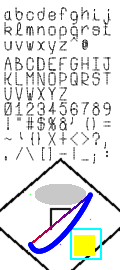
\includegraphics[width=5cm]{tga.png}
\end{center} 
	
\end{document}


